\documentclass[usenames,dvipsnames, 18pt, compress, aspectratio=169]{beamer}

% can be compiled by xelatex -shell-escape presentation.tex

\usetheme[]{m}

\usepackage[utf8]{inputenc}
\usepackage[russian, english]{babel}
\usepackage{booktabs}
\usepackage[scale=2]{ccicons}
\usepackage{listings}
\usepackage{marvosym}
\usepackage{color}
\usepackage{xcolor}
\usepackage[document]{ragged2e}
\usepackage[export]{adjustbox}
\usepackage{fontawesome}
\usepackage{enumitem}
\usepackage{minted}
\usemintedstyle{tango}
\usepackage[normalem]{ulem}
\usepackage{tikz}
\usetikzlibrary{mindmap}
\usepackage{graphicx}
\usepackage{eso-pic}
\usepackage{verbatim}
\usepackage{smartdiagram}
\usesmartdiagramlibrary{additions}
\usetikzlibrary{trees}
\usepackage{datetime}

%\usemintedstyle{monokai}

\usetikzlibrary{shapes,arrows,positioning}
\graphicspath{{images/}}
\newfontfamily{\FA}{FontAwesome}

\definecolor{check}{rgb}{0.1,2,0.3}
\definecolor{fail}{rgb}{2,0.1,0.1}
\definecolor{question}{rgb}{0.9,0.9,0.0}

\def\twitter{{\FA \faTwitter}}
\def\github{{\FA \faGithub}}
\def\email{{\FA \faEnvelope}}
\def\check{\textcolor{check}{\FA \faCheck}}
\def\fail{\textcolor{fail}{\FA \faRemove}}
\def\question{\textcolor{question}{\FA \faSearch}}

\renewcommand{\ttdefault}{pcr}
\newfontfamily{\ttfamily}{Fira Code}

\usefonttheme{professionalfonts} % using non standard fonts for beamer
\usefonttheme{serif} % default family is serif
\usepackage{fontspec}
\setmainfont{Liberation Sans}
%\setsansfont[BoldItalicFont={Liberation Sans}, ItalicFont={Liberation Sans}, BoldFont={Liberation Sans}]{Liberation Sans}
\newfontfamily\ExtraLight{Liberation Sans}
\newfontfamily\Light{Liberation Sans}
\newfontfamily\Book{Liberation Sans}
\newfontfamily\Medium{Liberation Sans}

\makeatletter
\newcommand\HUGE{\@setfontsize\Huge{32}{41}}
\makeatother

\newcommand\AtPagemyUpperLeft[1]{\AtPageLowerLeft{%
\put(\LenToUnit{0.85\paperwidth},\LenToUnit{0.05\paperheight}){#1}}}

\newcommand\AtPagemyUpperTop[1]{\AtPageLowerLeft{%
\put(\LenToUnit{0.42\paperwidth},\LenToUnit{0.90\paperheight}){#1}}}

\renewcommand{\ULthickness}{2.0pt}

\definecolor{links}{HTML}{0099FF}
\hypersetup{colorlinks, linkcolor=, urlcolor=links}

\setbeamerfont{section title}{family=\Book, size=\Huge, shape=\normalfont}
\setbeamerfont{frametitle}{family=\Book, size=\large, shape=\normalfont}
\setbeamerfont{title}{family=\Book, size=\Large, shape=\normalfont}
\setbeamerfont{subtitle}{size=\small}
\setbeamerfont{author}{family=\ExtraLight, size=\footnotesize}

\newdateformat{specialdate}{\twodigit{\THEDAY}-\twodigit{\THEMONTH}-\THEYEAR}

\setbeamertemplate{title page}
{

  %\AddToShipoutPictureFG*{
      %\AtPagemyUpperTop{{
\includegraphics[width=2.0cm,keepaspectratio]{logo.png}}}
  %}%

  \vspace*{2.1cm}
  \begin{minipage}[b][\paperheight]{\textwidth}
  \begin{center}

    \ifx\inserttitle\@empty\else
    {{% \inserttitle is nonempty
      \raggedright%
      %\linespread{1.0}%
      \usebeamerfont{title}%
      \usebeamercolor[fg]{title}%
      %\vspace*{1.3em}
      \if@noSmallCapitals%
        \inserttitle%
      \else%
        \scshape{\color{black} \textbf{\begin{center}NOSQL FOR\\POSTGRESQL\end{center}}}%
      \fi%
      \vspace*{0.3em}
    }}
    \fi

    %\begin{tikzpicture}
        %\fill[color=orange] (3cm, \paperheight-6pt) rectangle (\paperwidth-3cm,\paperheight);
    %\end{tikzpicture}

    \vspace*{0.5em}%

    \ifx\insertsubtitle\@empty\else
    {{% \insertsubtitle is nonempty
      \usebeamerfont{subtitle}%
      \usebeamercolor[fg]{subtitle}%
      {\color{black} \insertsubtitle}%
      \vspace*{3.0em}%
    }}
    \fi

    \vspace*{1.0em}%

    \usebeamerfont{author}%
    \usebeamercolor[fg]{author}%
    {\color{black} \insertauthor}%

    \vspace*{1.5em}
    \fontsize{8pt}{10}\selectfont
    {\color{black} 09-27-2017}%

    \vfill
    \vspace*{2em}
  \end{center}
  \end{minipage}
}

\setbeamertemplate{section page}
{
  \vspace{2em}
  \centering
  \begin{minipage}{22em}
    \usebeamercolor[fg]{section title}
    \usebeamerfont{section title}
    {\color{black} \insertsectionhead\\[-1ex]}
  \end{minipage}
  \par
}

\setbeamertemplate{footline}
{
\begin{beamercolorbox}[wd=\textwidth,ht=3ex,dp=3ex,leftskip=0.3cm,rightskip=0.3cm]{structure}
  \usebeamerfont{page number in head/foot}
  \insertframenumber
\end{beamercolorbox}
}

\title{NOSQL INSIDE SQL}
\subtitle{BEST PRACTICES}
\date{\today}
\author{DMITRY DOLGOV}
\institute{}

\begin{document}
{
  \usebackgroundtemplate{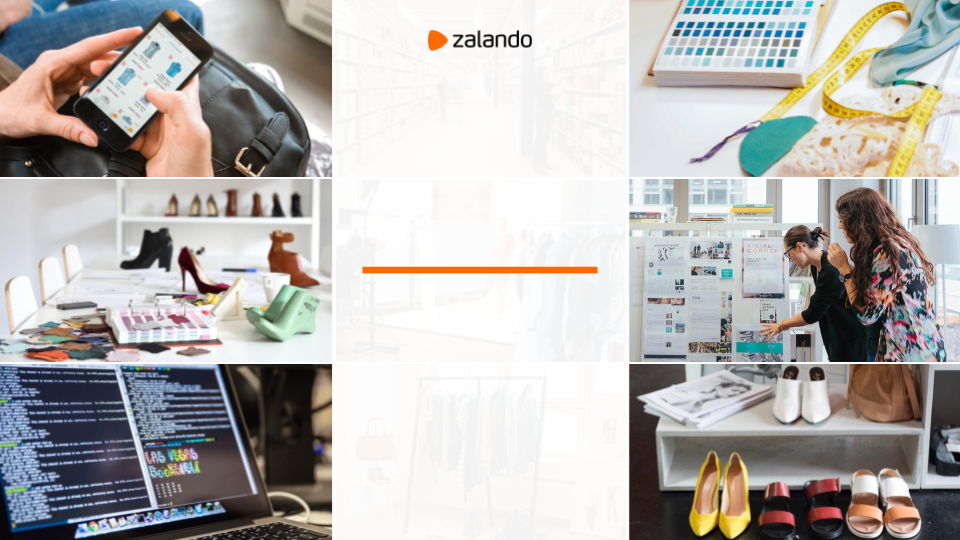
\includegraphics[width=\paperwidth]{template.png}}%
  \fontsize{17pt}{18}\selectfont
  \maketitle
}

\fontsize{17pt}{19}\selectfont
\section{}


\AddToShipoutPictureBG{
  \AtPagemyUpperLeft{{
\includegraphics[width=2.0cm,keepaspectratio]{logo.png}}}
}%

\setbeamertemplate{background canvas}{
\begin{tikzpicture}
    \clip (0,0) rectangle (\paperwidth,\paperheight);
    \fill[color=orange] (4cm, \paperheight-6pt) rectangle (\paperwidth-4cm,\paperheight);
\end{tikzpicture}
}

\fontsize{17pt}{19}\selectfont
\begin{frame}
    \frametitle{}
    \begin{center}

    \vspace{0.5cm}
    \begin{figure}
        
\includegraphics[width=0.5\textwidth,center]{approved.png}
    \end{figure}

    \end{center}
\end{frame}

\begin{frame}
    \frametitle{}
    \begin{center}
        \pause
        \begin{itemize}[label={\MVRightarrow}]
            \item <+-> Jsonb internals and performance-related factors
            \item <+-> Tricky queries
            \item <+-> Benchmarks
            \item <+-> How to shoot yourself in the foot
        \end{itemize}
    \end{center}
\end{frame}

\fontsize{13pt}{14}\selectfont
\section{Internals}
\fontsize{17pt}{18}\selectfont

\begin{frame}
    \frametitle{}
    \begin{center}
        \textbf{Performance-related factors}
        \pause
        \begin{itemize}[label={\MVRightarrow}]
            \item <+-> On-disk representation
            \item <+-> In-memory representation
            \item <+-> Indexing support
        \end{itemize}
    \end{center}
\end{frame}
\note{
    оптимизация по размеру и пробеганию
}

\fontsize{17pt}{19}\selectfont
\begin{frame}
    \frametitle{}
    \begin{center}

    \begin{figure}
        
\includegraphics[width=0.8\textwidth,center]{fry_disk_json2.jpg}
    \end{figure}

    \end{center}
\end{frame}

\fontsize{14pt}{16}\selectfont
\begin{frame}
    \frametitle{}
    \begin{center}
    \tikzstyle{every node}=[
        draw=gray,
        thick,
        anchor=west,
        rounded corners,
        top color=gray!7,
        bottom color=gray!7,
        minimum width=2cm,
        minimum height=1cm,
    ]
    \tikzstyle{empty}=[
        draw=gray,
        thick,
        anchor=west,
        rounded corners,
        top color=gray!7,
        bottom color=gray!7,
        minimum width=0cm,
        minimum height=0cm,
    ]
    \tikzstyle{selected}=[draw=red,fill=red!30]
    \tikzstyle{optional}=[dashed,fill=gray!50]
    \begin{tikzpicture}[%
      grow via three points={one child at (0.5,-1.2) and
      two children at (0.5,-1.2) and (0.5,-2.4)},
      edge from parent path={(\tikzparentnode.south) |- (\tikzchildnode.west)}]
      \node {{Jsonb}}
        child { node {{document size}}}
        child { node {{node}}
          child { node {{node}}
              child { node {{JEntry}}}
              child { node {{content}}}
          }
          child { node [empty] {...}}
        };
    \end{tikzpicture}

    \end{center}
\end{frame}

\fontsize{14pt}{16}\selectfont
\begin{frame}
    \frametitle{}
    \begin{center}
    \tikzstyle{every node}=[
        draw=gray,
        thick,
        anchor=west,
        rounded corners,
        top color=gray!7,
        bottom color=gray!7,
        minimum width=2cm,
        minimum height=1cm,
    ]
    %\tikzstyle{selected}=[
        %draw=gray,
        %thick,
        %anchor=west,
        %rounded corners,
        %top color=red!7,
        %bottom color=red!7,
        %fill=red,
        %minimum width=2cm,
        %minimum height=1cm,
    %]
    \tikzstyle{empty}=[
        draw=gray,
        thick,
        anchor=west,
        rounded corners,
        top color=gray!7,
        bottom color=gray!7,
        minimum width=0cm,
        minimum height=0cm,
    ]
    \tikzstyle{selected}=[draw=red,fill=red!30]
    \tikzstyle{optional}=[dashed,fill=gray!50]
    \begin{tikzpicture}[%
      grow via three points={one child at (0.5,-1.2) and
      two children at (0.5,-1.2) and (0.5,-2.4)},
      edge from parent path={(\tikzparentnode.south) |- (\tikzchildnode.west)}]
      \node {{Jsonb}}
        child { node {{document size}}}
        child { node {{node}}
          child { node [color=red!45, text=black, top color=red!25, bottom color=red!25] {{node}}
              child { node [color=red!45, text=black, top color=red!25, bottom color=red!25] {{JEntry}}}
              child { node {{content}}}
          }
          child { node [empty] {...}}
        };
    \end{tikzpicture}

    \end{center}
\end{frame}

\fontsize{14pt}{16}\selectfont
\begin{frame}
    \frametitle{}
    \begin{center}
    \tikzstyle{every node}=[
        draw=gray,
        thick,
        anchor=west,
        rounded corners,
        top color=gray!7,
        bottom color=gray!7,
        minimum width=2cm,
        minimum height=1cm,
    ]
    \tikzstyle{empty}=[
        draw=gray,
        thick,
        anchor=west,
        rounded corners,
        top color=gray!7,
        bottom color=gray!7,
        minimum width=0cm,
        minimum height=0cm,
    ]
    \tikzstyle{selected}=[draw=red,fill=red!30]
    \tikzstyle{optional}=[dashed,fill=gray!50]
    \begin{tikzpicture}[%
      grow via three points={one child at (0.5,-1.2) and
      two children at (0.5,-1.2) and (0.5,-2.4)},
      edge from parent path={(\tikzparentnode.south) |- (\tikzchildnode.west)}]
      \node {{Jsonb Header}}
        child { node {{type}}}
        child { node {{number of items}}}
        child { node {{JEntry}}
            child { node {{length or offset?}}}
            child { node {{value type}}}
            child { node {{value length or offset}}}
        };
    \end{tikzpicture}

    \end{center}
\end{frame}

\begin{frame}
    \frametitle{}
    \begin{center}
    \textbf{JB\_OFFSET\_STRIDE}

    \begin{itemize}[label={\MVRightarrow}]
        \item JEntry may contains a value lenght or offset
        \item Offset = access speed
        \item Length = compressibility
        \item Every \textbf{JB\_OFFSET\_STRIDE}'th JEntry contains an offset
        \item Rest of them contain length
    \end{itemize}
    \end{center}
\end{frame}

\tikzset{every shadow/.style={fill=none,shadow scale=0}}

\fontsize{14pt}{16}\selectfont
\begin{frame}
    \frametitle{}
    \begin{center}
    \tikzstyle{every node}=[
        draw=gray,
        thick,
        anchor=west,
        rounded corners,
        top color=gray!7,
        bottom color=gray!7,
        minimum width=2cm,
        minimum height=1cm,
    ]
    \tikzstyle{empty}=[
        draw=gray,
        thick,
        anchor=west,
        rounded corners,
        top color=gray!7,
        bottom color=gray!7,
        minimum width=0cm,
        minimum height=0cm,
    ]
    \tikzstyle{selected}=[draw=red,fill=red!30]
    \tikzstyle{optional}=[dashed,fill=gray!50]
    \begin{tikzpicture}[%
      grow via three points={one child at (0.5,-1.2) and
      two children at (0.5,-1.2) and (0.5,-2.4)},
      edge from parent path={(\tikzparentnode.south) |- (\tikzchildnode.west)}]
      \node {{Bson}}
        child { node {{document size}}}
        child { node {{node}}
          child { node {{node}}
              child { node {{Header}}}
              child { node {{Content}}}
          }
          child { node [empty] {...}}
        };
    \end{tikzpicture}

    \end{center}
\end{frame}

\fontsize{14pt}{16}\selectfont
\begin{frame}
    \frametitle{}
    \begin{center}
    \tikzstyle{every node}=[
        draw=gray,
        thick,
        anchor=west,
        rounded corners,
        top color=gray!7,
        bottom color=gray!7,
        minimum width=2cm,
        minimum height=1cm,
    ]
    \tikzstyle{empty}=[
        draw=gray,
        thick,
        anchor=west,
        rounded corners,
        top color=gray!7,
        bottom color=gray!7,
        minimum width=0cm,
        minimum height=0cm,
    ]
    \tikzstyle{selected}=[draw=red,fill=red!30]
    \tikzstyle{optional}=[dashed,fill=gray!50]
    \begin{tikzpicture}[%
      grow via three points={one child at (0.5,-1.2) and
      two children at (0.5,-1.2) and (0.5,-2.4)},
      edge from parent path={(\tikzparentnode.south) |- (\tikzchildnode.west)}]
      \node {{Bson}}
        child { node {{document size}}}
        child { node {{node}}
          child { node {{node}}
              child { node [color=red!45, text=black, top color=red!25, bottom color=red!25] {{Header}}}
              child { node {{Content}}}
          }
          child { node [empty] {...}}
        };
    \end{tikzpicture}

    \end{center}
\end{frame}

\fontsize{14pt}{16}\selectfont
\begin{frame}
    \frametitle{}
    \begin{center}
    \tikzstyle{every node}=[
        draw=gray,
        thick,
        anchor=west,
        rounded corners,
        top color=gray!7,
        bottom color=gray!7,
        minimum width=2cm,
        minimum height=1cm,
    ]
    \tikzstyle{empty}=[
        draw=gray,
        thick,
        anchor=west,
        rounded corners,
        top color=gray!7,
        bottom color=gray!7,
        minimum width=0cm,
        minimum height=0cm,
    ]
    \tikzstyle{selected}=[draw=red,fill=red!30]
    \tikzstyle{optional}=[dashed,fill=gray!50]
    \begin{tikzpicture}[%
      grow via three points={one child at (0.5,-1.2) and
      two children at (0.5,-1.2) and (0.5,-2.4)},
      edge from parent path={(\tikzparentnode.south) |- (\tikzchildnode.west)}]
      \node {{Bson Header}}
        child { node {{Value type}}}
        child { node {{Key name}}}
        child { node {{Value size}}};
    \end{tikzpicture}

    \end{center}
\end{frame}

\fontsize{14pt}{16}\selectfont
\begin{frame}
    \frametitle{}
    \begin{center}
    \tikzstyle{every node}=[
        draw=gray,
        thick,
        anchor=west,
        rounded corners,
        top color=gray!7,
        bottom color=gray!7,
        minimum width=2cm,
        minimum height=1cm,
    ]
    \tikzstyle{empty}=[
        draw=gray,
        thick,
        anchor=west,
        rounded corners,
        top color=gray!7,
        bottom color=gray!7,
        minimum width=0cm,
        minimum height=0cm,
    ]
    \tikzstyle{selected}=[draw=red,fill=red!30]
    \tikzstyle{optional}=[dashed,fill=gray!50]
    \begin{tikzpicture}[%
      grow via three points={one child at (0.5,-1.2) and
      two children at (0.5,-1.2) and (0.5,-2.4)},
      edge from parent path={(\tikzparentnode.south) |- (\tikzchildnode.west)}]
      \node {{MySQL Json}}
        child { node {{node}}
          child { node {{node}}
              child { node {{Type}}}
              child { node {{Value}}}
          }
          child { node [empty] {...}}
        };
    \end{tikzpicture}

    \end{center}
\end{frame}

\fontsize{14pt}{16}\selectfont
\begin{frame}
    \frametitle{}
    \begin{center}
    \tikzstyle{every node}=[
        draw=gray,
        thick,
        anchor=west,
        rounded corners,
        top color=gray!7,
        bottom color=gray!7,
        minimum width=2cm,
        minimum height=1cm,
    ]
    \tikzstyle{empty}=[
        draw=gray,
        thick,
        anchor=west,
        rounded corners,
        top color=gray!7,
        bottom color=gray!7,
        minimum width=0cm,
        minimum height=0cm,
    ]
    \tikzstyle{selected}=[draw=red,fill=red!30]
    \tikzstyle{optional}=[dashed,fill=gray!50]
    \begin{tikzpicture}[%
      grow via three points={one child at (0.5,-1.2) and
      two children at (0.5,-1.2) and (0.5,-2.4)},
      edge from parent path={(\tikzparentnode.south) |- (\tikzchildnode.west)}]
      \node {{MySQL Json}}
        child { node {{node}}
          child { node {{node}}
              child { node {{Type}}}
              child { node [color=red!45, text=black, top color=red!25, bottom color=red!25]{{Value}}}
          }
          child { node [empty] {...}}
        };
    \end{tikzpicture}

    \end{center}
\end{frame}

\fontsize{14pt}{16}\selectfont
\begin{frame}
    \frametitle{}
    \begin{center}
    \tikzstyle{every node}=[
        draw=gray,
        thick,
        anchor=west,
        rounded corners,
        top color=gray!7,
        bottom color=gray!7,
        minimum width=2cm,
        minimum height=1cm,
    ]
    \tikzstyle{empty}=[
        draw=gray,
        thick,
        anchor=west,
        rounded corners,
        top color=gray!7,
        bottom color=gray!7,
        minimum width=0cm,
        minimum height=0cm,
    ]
    \tikzstyle{selected}=[draw=red,fill=red!30]
    \tikzstyle{optional}=[dashed,fill=gray!50]
    \begin{tikzpicture}[%
      grow via three points={one child at (0.5,-1.2) and
      two children at (0.5,-1.2) and (0.5,-2.4)},
      edge from parent path={(\tikzparentnode.south) |- (\tikzchildnode.west)}]
      \node {{MySQL Json Object}}
        child { node {{Count of elements}}}
        child { node {{Size}}}
        child { node {{Pointers to keys}}}
        child { node {{Pointers to values}}}
        child { node {{Keys}}}
        child { node {{Values}}};
    \end{tikzpicture}

    \end{center}
\end{frame}
\note{
    Json value can be inlined (so, without pointer), if
    it's a literal of small integer. All values are at the end
    independently from nesting level (for PG all values for one
    nesting level are at the end).
}

\fontsize{14pt}{16}\selectfont
\begin{frame}
    \frametitle{}
    \begin{center}
    \tikzstyle{every node}=[
        draw=gray,
        thick,
        anchor=west,
        rounded corners,
        top color=gray!7,
        bottom color=gray!7,
        minimum width=2cm,
        minimum height=0.5cm,
    ]
    \tikzstyle{empty}=[
        draw=gray,
        thick,
        anchor=west,
        rounded corners,
        top color=gray!7,
        bottom color=gray!7,
        minimum width=0cm,
        minimum height=0cm,
    ]
    \tikzstyle{selected}=[draw=red,fill=red!30]
    \tikzstyle{optional}=[dashed,fill=gray!50]

    \begin{columns}[T,onlytextwidth]
    \column{0.1\textwidth}
    \column{0.4\textwidth}
    \begin{tikzpicture}[%
      grow via three points={one child at (0.5,-1.0) and
      two children at (0.5,-1.0) and (0.5,-2.0)},
      edge from parent path={(\tikzparentnode.south) |- (\tikzchildnode.west)}]
      \node {{Bson}}
        child { node {{Key}}}
        child { node {{Value}}
          child { node {{Key}}}
          child { node {{Value}}}
        }
        child [missing] {}
        child [missing] {}
        child { node {{Key}}}
        child { node {{Value}}}
        child { node [empty] {...}};
    \end{tikzpicture}

    \column{0.4\textwidth}
    \begin{tikzpicture}[%
      grow via three points={one child at (0.5,-1.0) and
      two children at (0.5,-1.0) and (0.5,-2.0)},
      edge from parent path={(\tikzparentnode.south) |- (\tikzchildnode.west)}]
      \node {{Jsonb/MySQL Json}}
        child { node {{Key}}}
        child { node {{Key}}}
        child { node {{Value}}
          child { node {{Key}}}
          child { node {{Value}}}
        }
        child [missing] {}
        child [missing] {}
        child { node {{Value}}}
        child { node [empty] {...}};
    \end{tikzpicture}
    \column{0.1\textwidth}
    \end{columns}

    \end{center}
\end{frame}
\note{
    MySQL - pointers, PG - implicit element order
}

\fontsize{17pt}{19}\selectfont
\begin{frame}
    \frametitle{}
    \begin{center}
    \inputminted[
        fontsize=\Large,
    ]{python}{sql/json_document.py}
    \end{center}
\end{frame}

\fontsize{17pt}{19}\selectfont
\begin{frame}
    \frametitle{}
    \begin{center}
    \inputminted[
        fontsize=\Large,
    ]{python}{sql/jsonb_binary.sql}

    \begin{figure}
        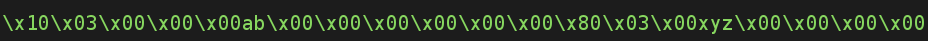
\includegraphics[width=1.0\textwidth,center]{jsonb_binary.png}
    \end{figure}

    \end{center}
\end{frame}

\begin{frame}
    \frametitle{}
    \begin{center}
    \inputminted[
        fontsize=\Large,
    ]{python}{sql/bson.py}

    \begin{figure}
        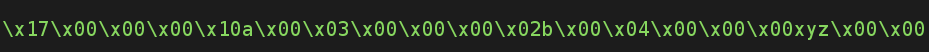
\includegraphics[width=1.0\textwidth,center]{bson_binary.png}
    \end{figure}

    \end{center}
\end{frame}

\begin{frame}
    \frametitle{}
    \begin{center}
    \inputminted[
        fontsize=\Large,
    ]{bash}{sql/mysql.sh}

    \begin{figure}
        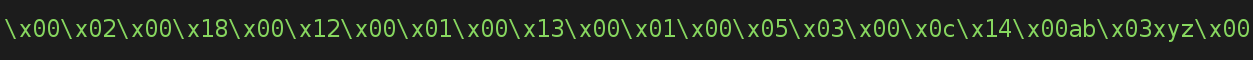
\includegraphics[width=1.0\textwidth,center]{mysql_binary.png}
    \end{figure}

    \end{center}
\end{frame}

\fontsize{14pt}{16}\selectfont
\begin{frame}
    \frametitle{}
    \begin{center}
    \textbf{TOAST}
    \vspace{20pt}

    \smartdiagramset{
        uniform color list=gray!10!gray!10 for 4 items,
        uniform arrow color=true,
        arrow color=black!70,
        back arrow disabled=true,
        module x sep=3.5cm,
        text width=2.5cm,
    }
    \smartdiagram[flow diagram:horizontal]{
        {Jsonb}, {Compression}, {Chunks}, {Toast table}
    }

    \vspace{20pt}
    \begin{itemize}[label={\MVRightarrow}]
        \item TOAST\_TUPLE\_THRESHOLD bytes (normally 2 kB)
        \item PostgreSQL and MySQL use LZ variation
        \item MongoDB uses snappy block compression
    \end{itemize}

    \end{center}
\end{frame}
\note{
    compression - mongodb - snappy
                - pg - lz variation
                - mysql - lz variation
}

\begin{frame}
    \frametitle{}
    \begin{center}
    \textbf{Alignment}

    \begin{itemize}[label={}]
        \item Variable-length portion is aligned to a 4-byte
        \item \inputminted[fontsize=\Large]{sql}{sql/insert_align1.sql}
        \item \begin{figure}
            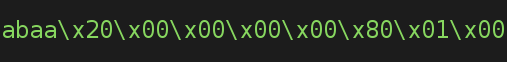
\includegraphics[width=0.58\textwidth,left]{align_short.png}
        \end{figure}

        \item \inputminted[fontsize=\Large]{sql}{sql/insert_align2.sql}
        \item \begin{figure}
            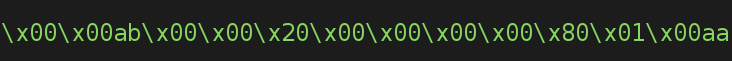
\includegraphics[width=0.75\textwidth,left]{align_long.png}
        \end{figure}

    \end{itemize}

    \end{center}
\end{frame}

\begin{frame}
    \frametitle{}
    \textbf{In-memory representation}
    \begin{center}
        \begin{itemize}[label={\MVRightarrow}]
            \item Tree-like representation (JsonbValue, Document, Json\_dom)
            \item Little bit more expensive but more convenient to work with
            \item Mostly in use to modify data (except MySQL)
            \item Most of the read operations use on-disk representation
        \end{itemize}
    \end{center}
\end{frame}

\begin{frame}
    \frametitle{}
    \textbf{Indexing support}
    \begin{center}
        \begin{itemize}[label={\MVRightarrow}]
            \item Postgresql -- single path, multiple paths, entire document
            \item MongoDB -- single path, multiple paths
            \item MySQL -- virtual columns, single path, multiple paths
        \end{itemize}
    \end{center}
\end{frame}
\note{
    entire document - all posible paths are indexed
    multiple fields - multicolumd index in postgresql, compount index in mongodb
}

\begin{frame}
    \frametitle{}
    \textbf{PG indexing details}
    \begin{center}
        \begin{itemize}[label={\MVRightarrow}]
            %\item JGIN\_MAXLENGTH
            \item jsonb\_path
            \item jsonb\_path\_ops
        \end{itemize}
    \end{center}
\end{frame}

\fontsize{13pt}{14}\selectfont
\section{Queries}
\fontsize{17pt}{18}\selectfont

\begin{frame}
    \frametitle{}
    \textbf{Pitfalls}
    \begin{center}
        \begin{itemize}[label={\MVRightarrow}]
            \item No Json path out of the box (jquery, SQL/JSON)
            \item Queries with an array somewhere in the middle
            \item Iterating through document
            \item Update inside document
        \end{itemize}
    \end{center}
\end{frame}

\fontsize{17pt}{19}\selectfont
\begin{frame}
    \frametitle{}
    \begin{center}
    \inputminted[
        fontsize=\Large,
    ]{json}{sql/with_array_data.json}
    \end{center}
\end{frame}

\fontsize{17pt}{19}\selectfont
\begin{frame}
    \frametitle{}
    \begin{center}
    \inputminted[
        fontsize=\Large,
    ]{sql}{sql/with_array.sql}
    \inputminted[
        fontsize=\large,
    ]{bash}{sql/with_array.sh}
    \end{center}
\end{frame}

\fontsize{17pt}{19}\selectfont
\begin{frame}
    \frametitle{}
    \begin{center}
    \inputminted[
        fontsize=\Large,
    ]{json}{sql/iterate_document_data.json}
    \end{center}
\end{frame}

\fontsize{17pt}{19}\selectfont
\begin{frame}
    \frametitle{}
    \begin{center}
    \inputminted[
        fontsize=\Large,
    ]{sql}{sql/iterate_document.sql}
    \inputminted[
        fontsize=\large,
    ]{bash}{sql/iterate_document.sh}
    \end{center}
\end{frame}

\fontsize{13pt}{14}\selectfont
\section{Benchmarks}
\fontsize{17pt}{18}\selectfont

\usebackgroundtemplate{
\includegraphics[width=\paperwidth]{great_performance3.jpg}}%
\begin{frame}
    \frametitle{}
\end{frame}

\setbeamertemplate{background canvas}{
\begin{tikzpicture}
    \clip (0,0) rectangle (\paperwidth,\paperheight);
    \fill[color=orange] (4cm, \paperheight-6pt) rectangle (\paperwidth-4cm,\paperheight);
\end{tikzpicture}
}
\begin{frame}
    \frametitle{}
    \begin{center}
        \textbf{AWS EC2}
        \begin{itemize}[label={}]
            \item m4.xlarge instance
            \item separate instance (database and generator)
            \item 16GB memory, 4 core 2.3GHz
            \item Ubuntu 16.04
            \item Same VPC and placement group
            \item AMI that supports HVM virtualization type
            \item at least 4 rounds of benchmark
        \end{itemize}
    \end{center}
\end{frame}

\begin{frame}
    \frametitle{}
    \begin{center}
        \begin{itemize}[label={}]
            \item PostgreSQL 9.6.3
            \item MySQL 5.7.9/8.0
            \item MongoDB 3.4.4
            \item YCSB 0.13
            \item $10^6$ rows and operations
            \item AWS EC2
        \end{itemize}
    \end{center}
\end{frame}

\begin{frame}
    \frametitle{}
    \begin{center}
        \textbf{Configuration}
        \begin{itemize}[label={}]
            \item shared\_buffers
            \item effective\_cache\_size
            \item max\_wal\_size
            \item innodb\_buffer\_pool\_size
            \item innodb\_log\_file\_size
            \item write concern level (journaled or transaction\_sync)
            \item checkpoint
            \item eviction
        \end{itemize}
    \end{center}
\end{frame}

\begin{frame}
    \frametitle{}
    \begin{center}
        \textbf{Document types}
        \begin{itemize}[label={}]
            \item “simple” document
            \item 10 key/value pairs (100 characters)
            \item
            \item “large” document
            \item 100 key/value pairs (200 characters)
            \item
            \item “complex” document
            \item 100 keys, 3 nesting levels (100 characters)
        \end{itemize}
    \end{center}
\end{frame}

\begin{frame}
    \frametitle{}
    \begin{center}
        \textbf{Select, GIN}
        \begin{itemize}[label={}]
            \item "simple" document
            \item jsonb\_path\_ops
            \item where data @> '\{"key": "value"\}'::jsonb
        \end{itemize}
    \end{center}
\end{frame}

\begin{frame}
    \frametitle{}
    \begin{center}
    \vspace{10pt}
    \begin{figure}
        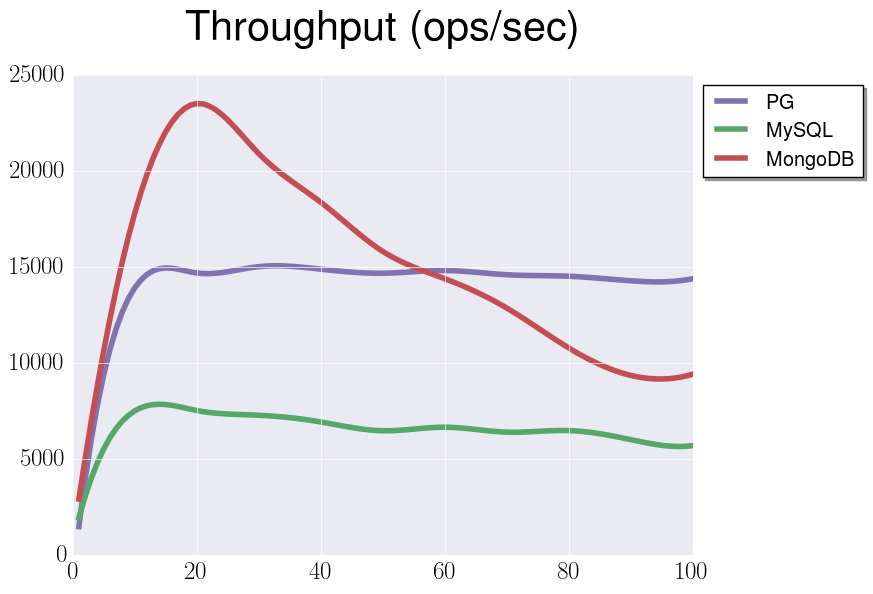
\includegraphics[width=0.8\textwidth,center]{benchmarks/select_jsonb_path_ops_throughput.png}
    \end{figure}
    \end{center}
\end{frame}

\begin{frame}
    \frametitle{}
    \begin{center}
    \vspace{10pt}
    \begin{figure}
        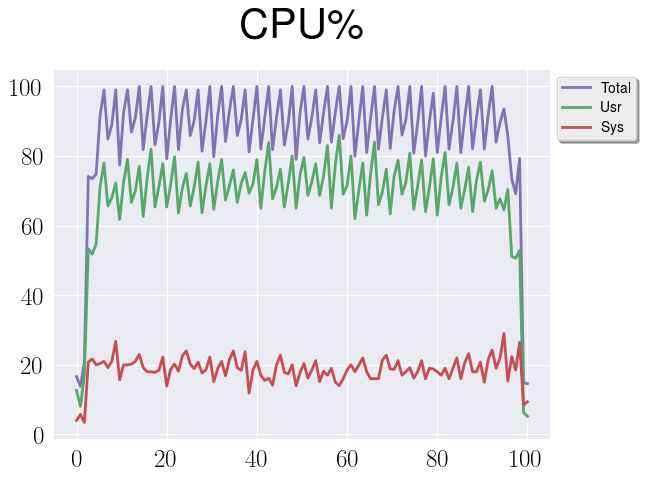
\includegraphics[width=0.75\textwidth,center]{benchmarks/pg_select_cpu_20.png}
    \end{figure}
    \end{center}
\end{frame}

\begin{frame}
    \frametitle{}
    \begin{center}
    \vspace{10pt}
    \begin{figure}
        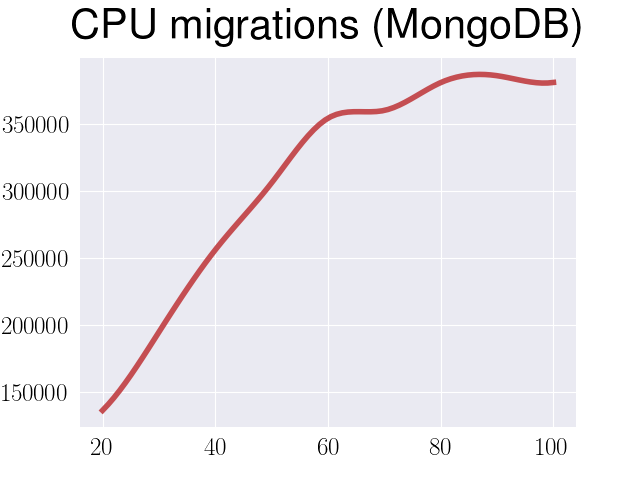
\includegraphics[width=0.75\textwidth,center]{benchmarks/mongodb_cpu_migrations.png}
    \end{figure}
    \end{center}
\end{frame}

\begin{frame}
    \frametitle{}
    \begin{center}
    \vspace{10pt}
    \begin{figure}
        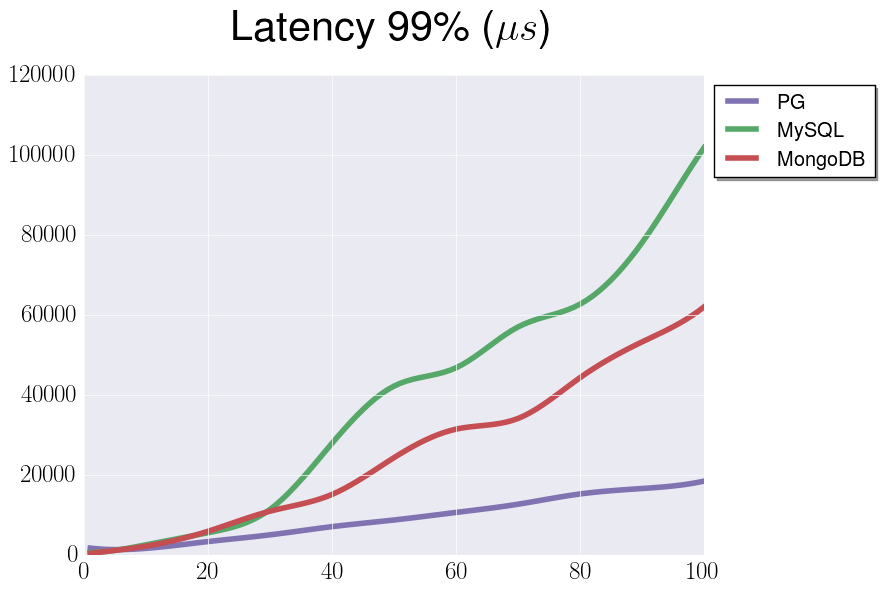
\includegraphics[width=0.8\textwidth,center]{benchmarks/select_jsonb_path_ops_latency_99.png}
    \end{figure}
    \end{center}
\end{frame}

\begin{frame}
    \frametitle{}
    \begin{center}
        \textbf{Select, BTree }
        \begin{itemize}[label={}]
            \item "simple" document
            \item btree
        \end{itemize}
    \end{center}
\end{frame}

\begin{frame}
    \frametitle{}
    \begin{center}
    \vspace{10pt}
    \begin{figure}
        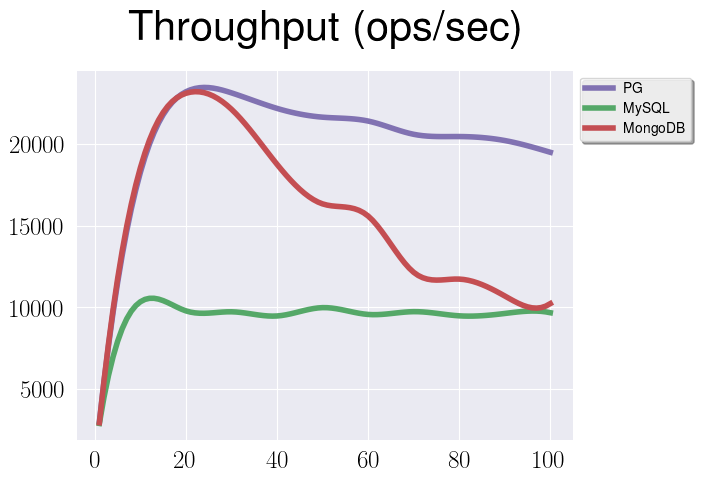
\includegraphics[width=0.8\textwidth,center]{benchmarks/select_btree_throughput.png}
    \end{figure}
    \end{center}
\end{frame}

%\begin{frame}
    %\frametitle{}
    %\begin{center}
    %%\vspace{-10pt}
    %\begin{figure}
        %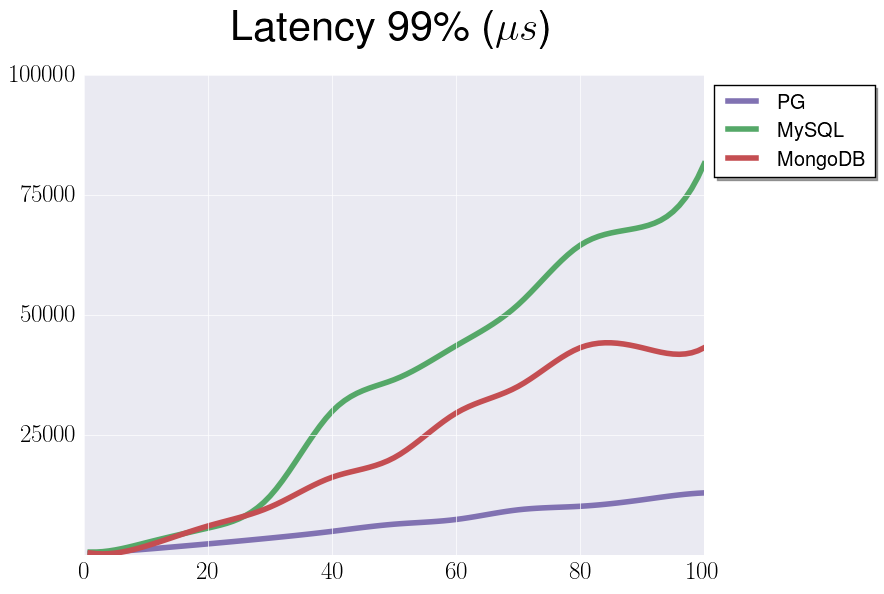
\includegraphics[width=0.75\textwidth,center]{benchmarks/select_btree_latency.png}
    %\end{figure}
    %\end{center}
%\end{frame}

\begin{frame}
    \frametitle{}
    \begin{center}
        \textbf{Select, BTree}
        \begin{itemize}[label={}]
            \item "complex" document
            \item btree
        \end{itemize}
    \end{center}
\end{frame}

\begin{frame}
    \frametitle{}
    \begin{center}
    \vspace{10pt}
    \begin{figure}
        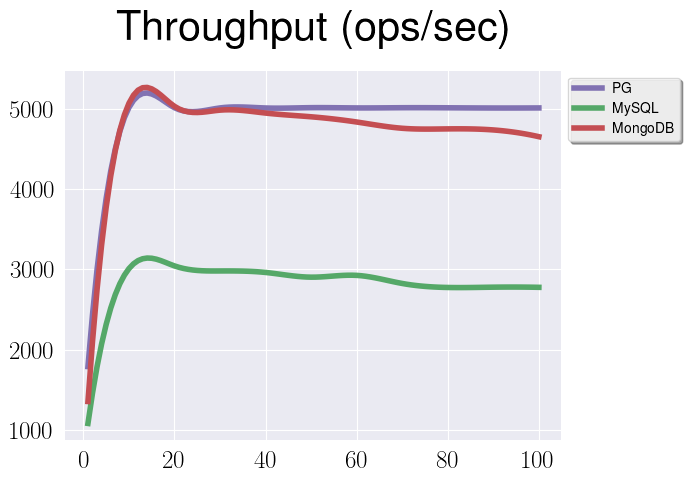
\includegraphics[width=0.8\textwidth,center]{benchmarks/select_complex_btree_throughput.png}
    \end{figure}
    \end{center}
\end{frame}

%\begin{frame}
    %\frametitle{}
    %\begin{center}
    %%\vspace{-10pt}
    %\begin{figure}
        %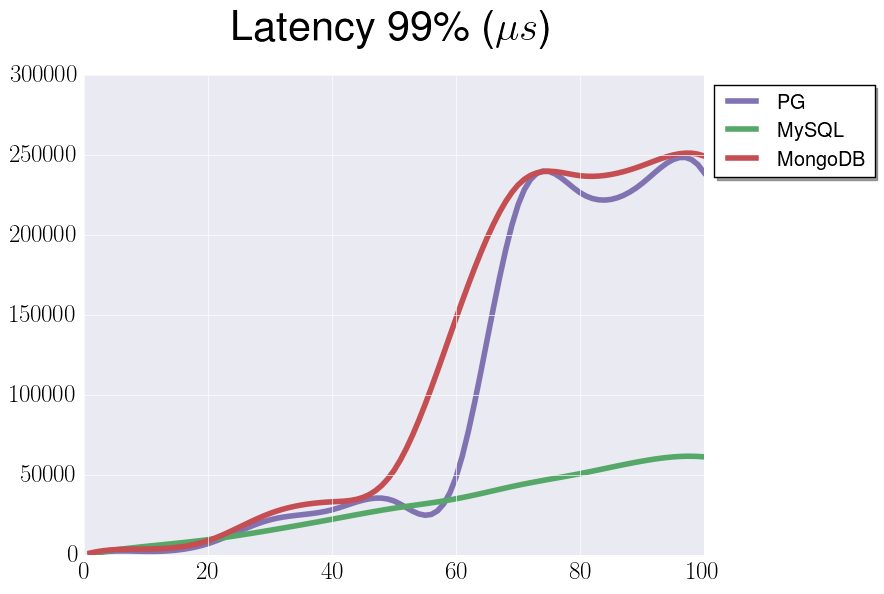
\includegraphics[width=0.75\textwidth,center]{benchmarks/select_complex_btree_latency_99.png}
    %\end{figure}
    %\end{center}
%\end{frame}

%\begin{frame}
    %\frametitle{}
    %\begin{center}
    %\vspace{-10pt}
    %\textbf{Простая выборка по ключу с индексом}
    %\begin{figure}
        %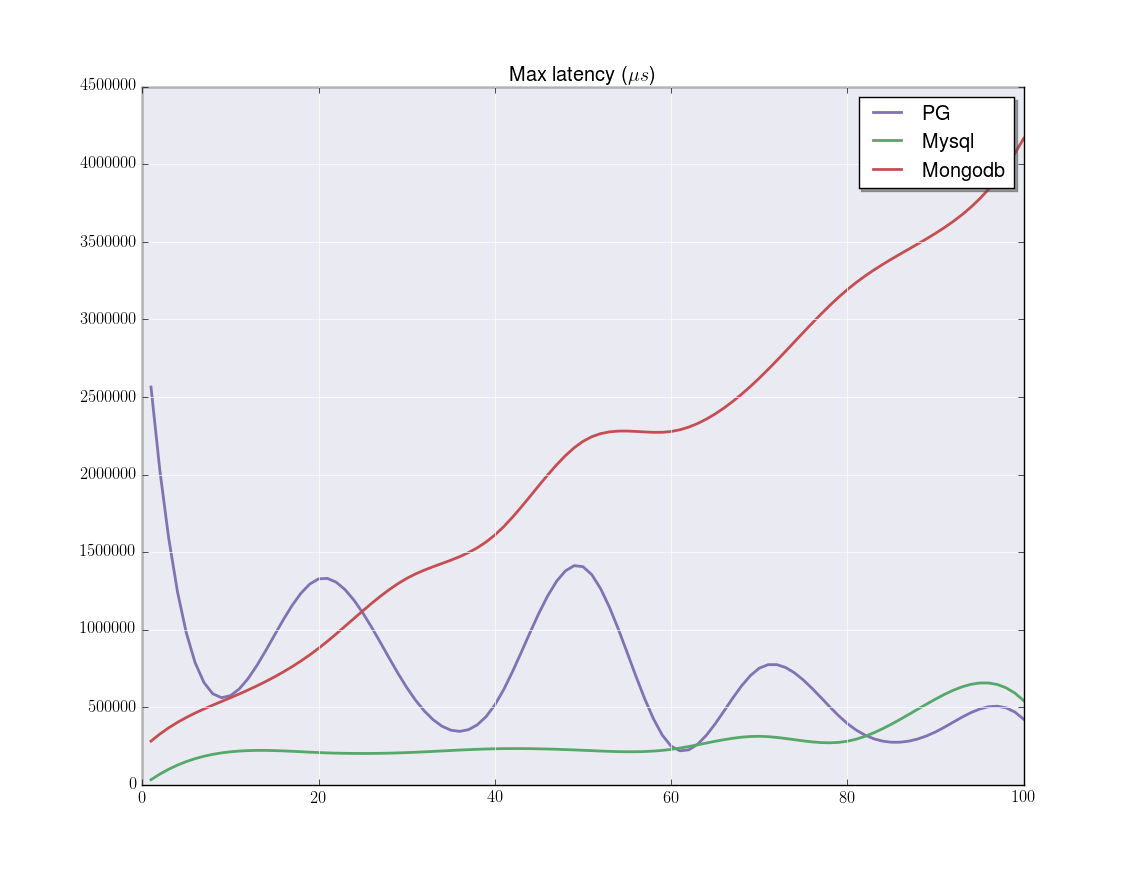
\includegraphics[width=0.7\textwidth,center]{benchmarks/simple_select_max_latency.png}
    %\end{figure}
    %\end{center}
%\end{frame}

%\begin{frame}
    %\frametitle{}
    %\begin{center}
    %%\vspace{-10pt}
    %\begin{figure}
        %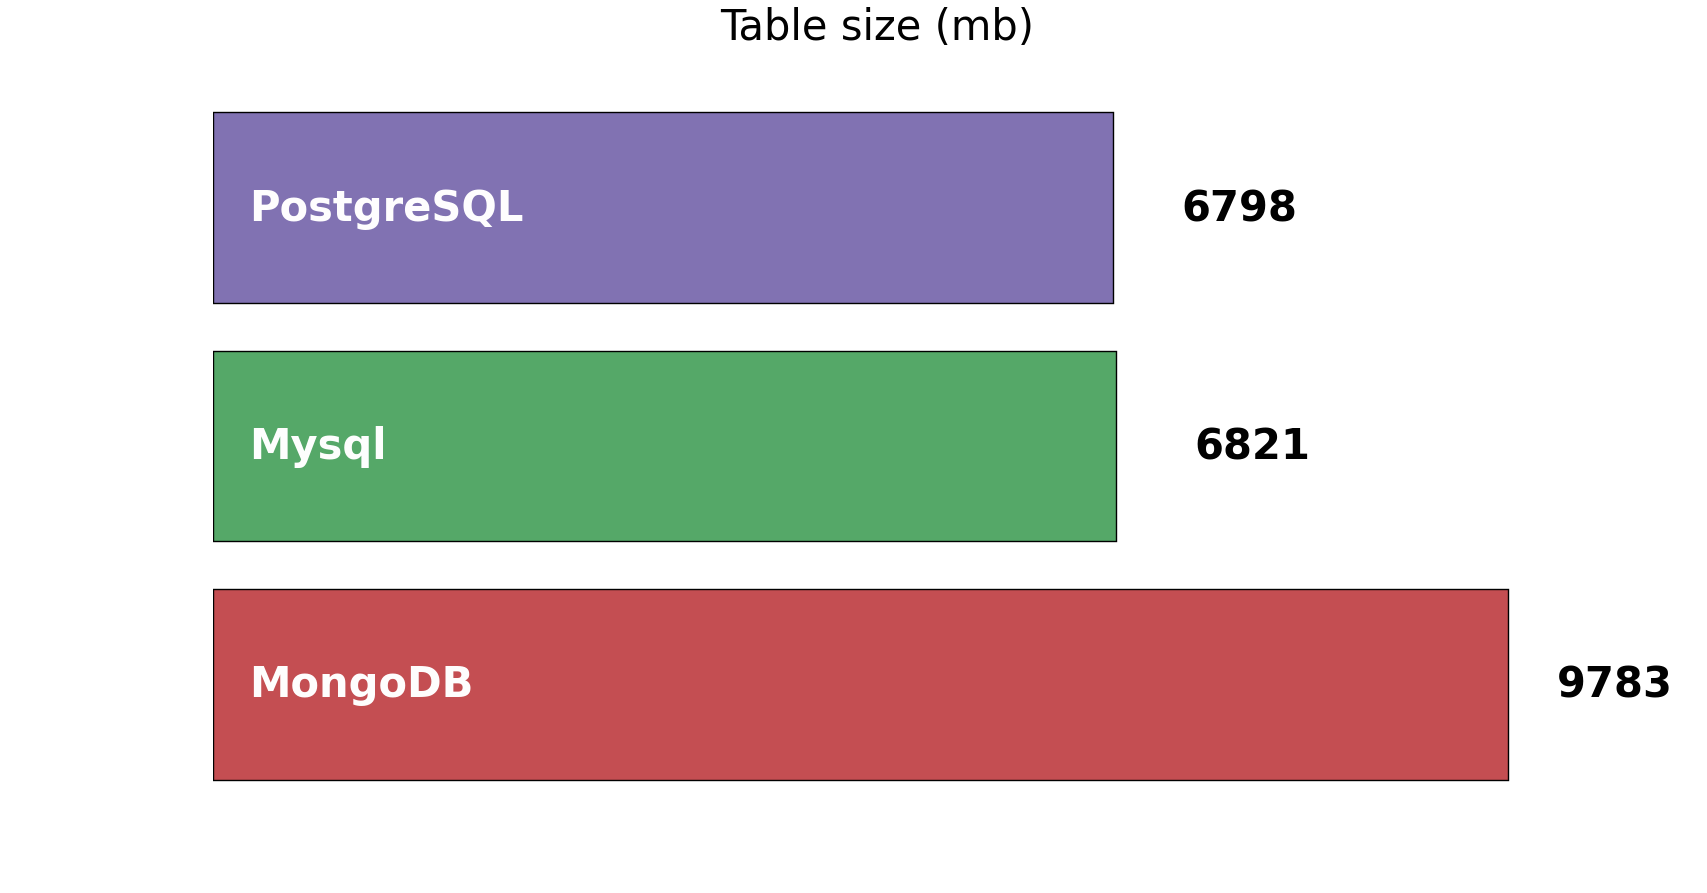
\includegraphics[width=0.95\textwidth,center]{benchmarks/table_size.png}
    %\end{figure}
    %\end{center}
%\end{frame}

%\begin{frame}
    %\frametitle{}
    %\begin{center}
    %\vspace{-10pt}
    %\textbf{Размер индексов}
    %\begin{figure}
        %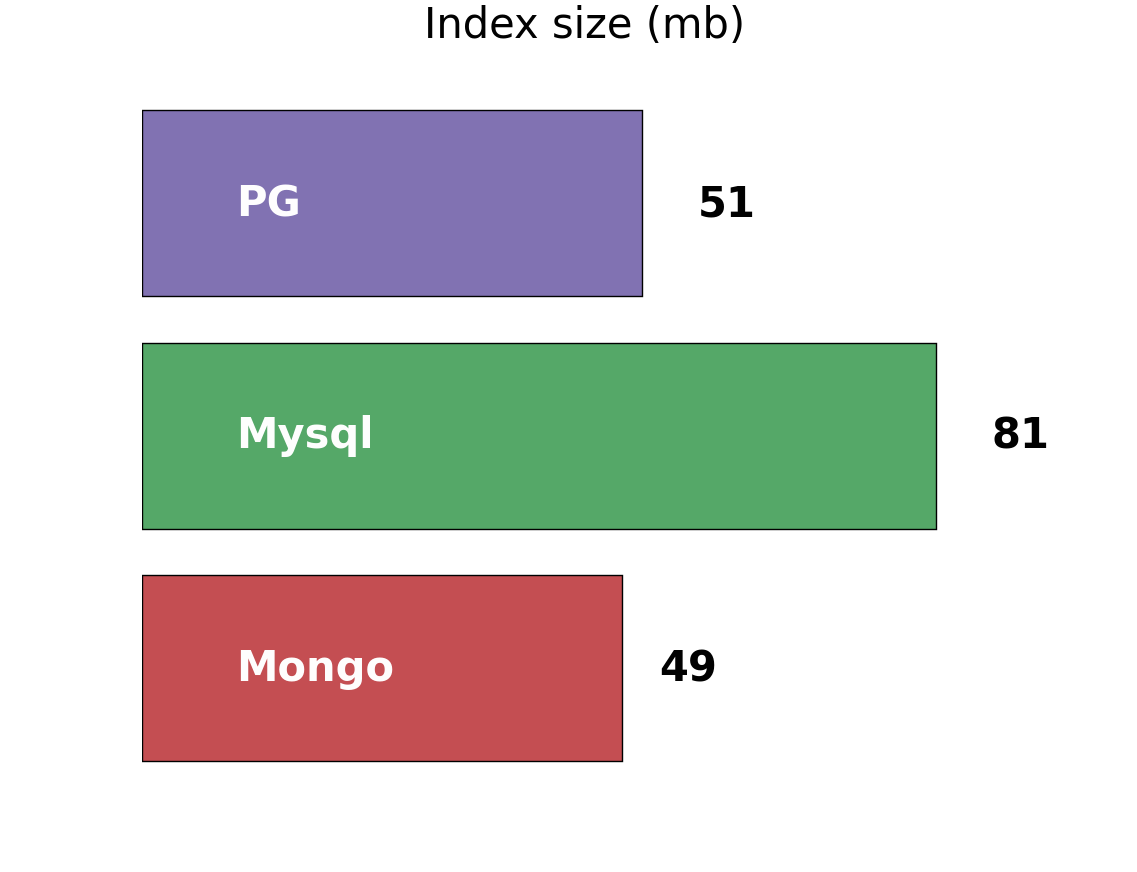
\includegraphics[width=0.7\textwidth,center]{benchmarks/index_size.png}
    %\end{figure}
    %\end{center}
%\end{frame}

%\begin{frame}
    %\frametitle{}
    %\begin{center}
    %\vspace{-10pt}
    %\textbf{Выборка документов с большим количеством ключей}
    %\end{center}
%\end{frame}
%\note{
    %сериализация в ширину
%}

%\begin{frame}
    %\frametitle{}
    %\begin{center}
    %\vspace{-10pt}
    %\textbf{Выборка документов с большой вложенностью}
    %\end{center}
%\end{frame}
%\note{
    %сериализация в глубину
%}

%\begin{frame}
    %\frametitle{}
    %\begin{center}
    %\vspace{-10pt}
    %\textbf{Выборка среза по документам}
    %\end{center}
%\end{frame}
%\note{
    %множественный detoast
%}

%\begin{frame}
    %\frametitle{}
    %\begin{center}
    %\vspace{-10pt}
    %\textbf{Выборка документов без кэша}
    %\end{center}
%\end{frame}
%\note{
    %моделирование ситуации, когда данные не влезают в память
    %и идет активная работа с диском
%}

%\begin{frame}
    %\frametitle{}
    %\begin{center}
    %\vspace{-10pt}
    %\textbf{SET STORAGE EXTERNAL}
    %\end{center}
%\end{frame}
%\note{
    %хранение jsonb в распакованном формате
%}

\begin{frame}
    \frametitle{}
    \begin{center}
        \textbf{Insert}
        \begin{itemize}[label={}]
            \item "simple" document
            \item journaled
        \end{itemize}
    \end{center}
\end{frame}

\begin{frame}
    \frametitle{}
    \begin{center}
    \vspace{10pt}
    \begin{figure}
        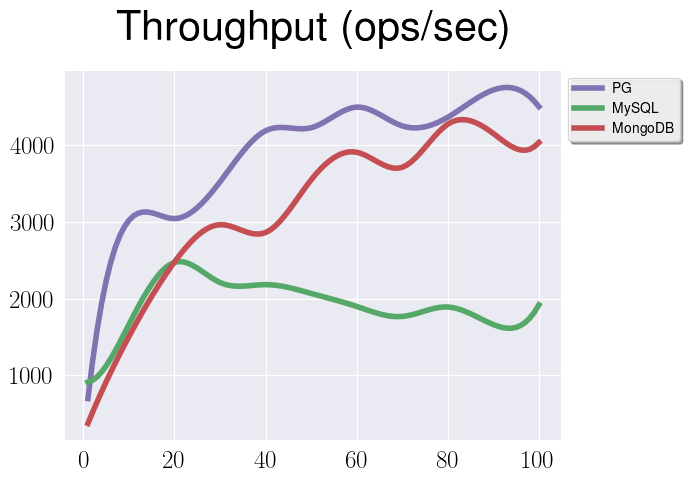
\includegraphics[width=0.8\textwidth,center]{benchmarks/insert_throughput_journaled2.png}
    \end{figure}
    \end{center}
\end{frame}

\begin{frame}
    \frametitle{}
    \begin{center}
    %\vspace{10pt}
    \begin{figure}
        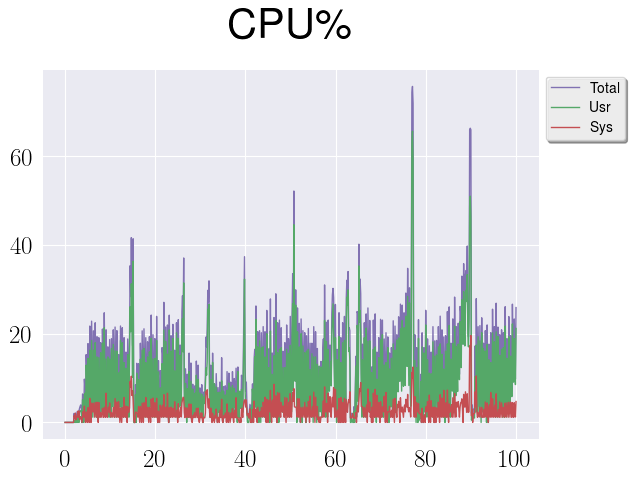
\includegraphics[width=0.8\textwidth,center]{benchmarks/mongodb_update_cpu_usage.png}
    \end{figure}
    \end{center}
\end{frame}

\begin{frame}
    \frametitle{}
    \begin{center}
    \vspace{10pt}
    \begin{figure}
        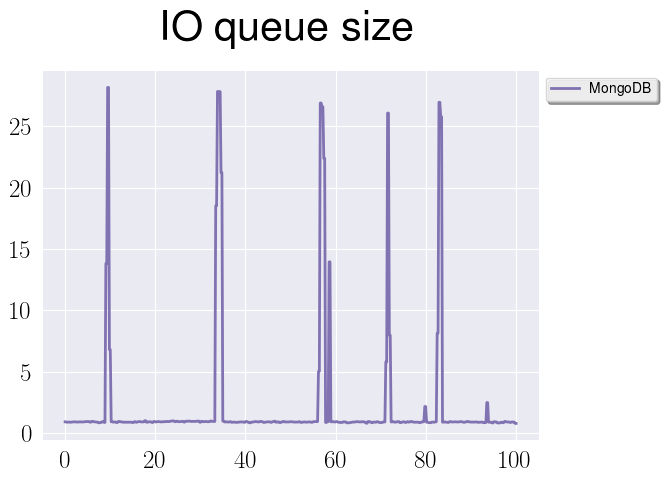
\includegraphics[width=0.8\textwidth,center]{benchmarks/mongodb_update_io_queue_size.png}
    \end{figure}
    \end{center}
\end{frame}

%\begin{frame}
    %\frametitle{}
    %\begin{center}
    %%\vspace{-10pt}
    %\begin{figure}
        %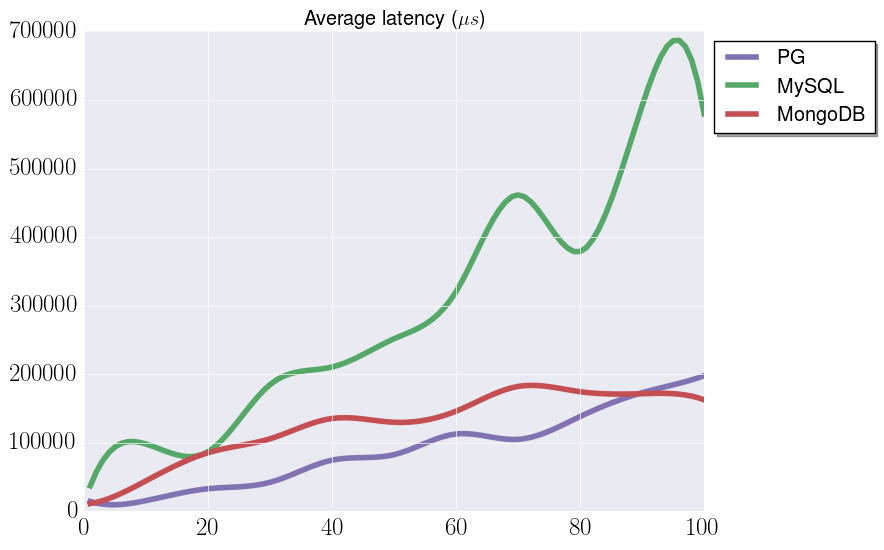
\includegraphics[width=0.75\textwidth,center]{benchmarks/insert_latency_99.png}
    %\end{figure}
    %\end{center}
%\end{frame}

\begin{frame}
    \frametitle{}
    \begin{center}
    \vspace{10pt}
    \begin{figure}
        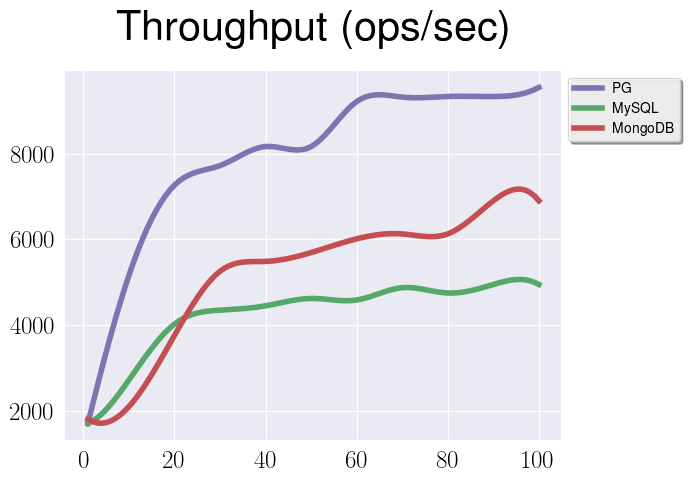
\includegraphics[width=0.8\textwidth,center]{benchmarks/insert_throughput_wal_size.png}
    \end{figure}
    \end{center}
\end{frame}

%\begin{frame}
    %\frametitle{}
    %\begin{center}
        %\textbf{Update 50\%, Select 50\%}
        %\begin{itemize}[label={}]
            %\item "simple" document
            %\item Update one field
            %\item transaction\_sync
        %\end{itemize}
    %\end{center}
%\end{frame}
%\note{checkpoints!}

%\begin{frame}
    %\frametitle{}
    %\begin{center}
    %%\vspace{-10pt}
    %\begin{figure}
        %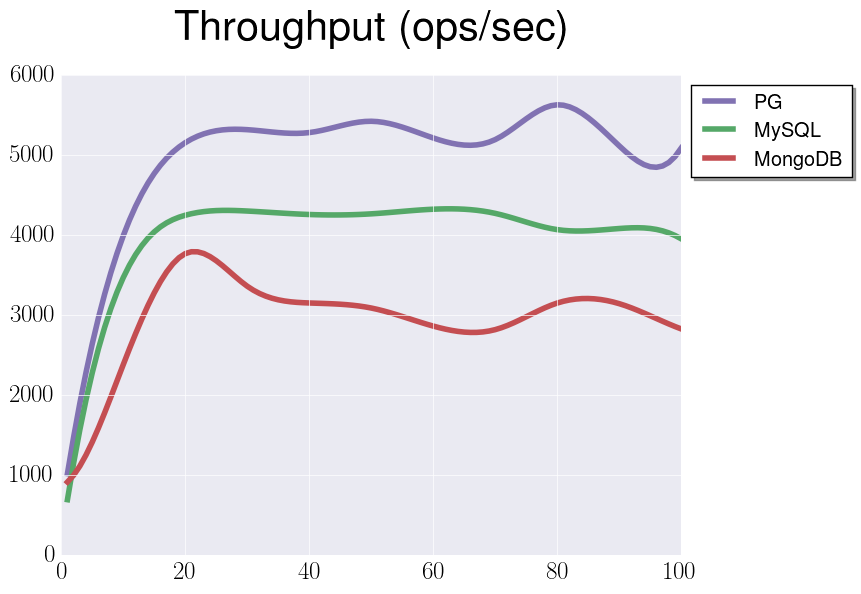
\includegraphics[width=0.75\textwidth,center]{benchmarks/update_btree_transaction_sync_throughput.png}
    %\end{figure}
    %\end{center}
%\end{frame}

%\begin{frame}
    %\frametitle{}
    %\begin{center}
    %%\vspace{-10pt}
    %\begin{figure}
        %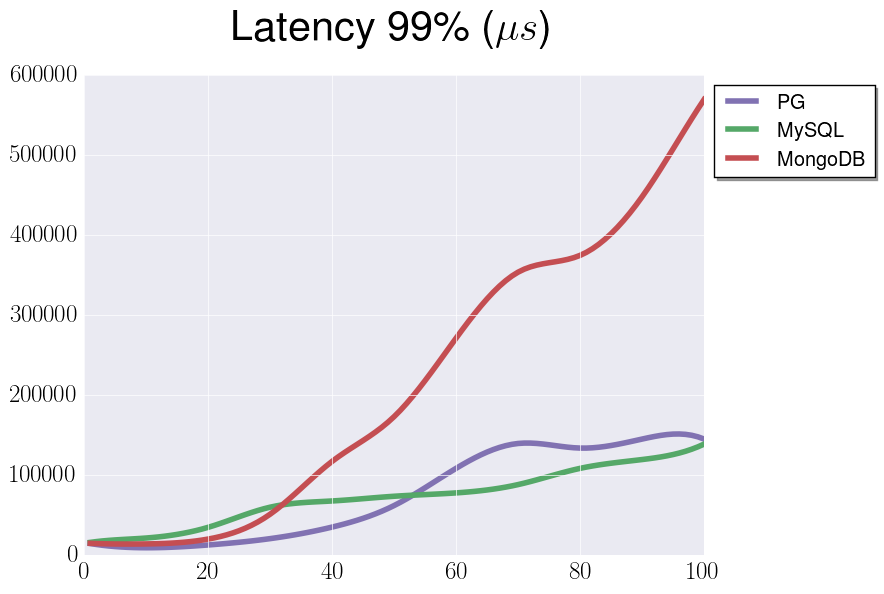
\includegraphics[width=0.75\textwidth,center]{benchmarks/update_btree_transaction_sync_latency.png}
    %\end{figure}
    %\end{center}
%\end{frame}

\begin{frame}
    \frametitle{}
    \begin{center}
        \textbf{Update 50\%, Select 50\%}
        \begin{itemize}[label={}]
            \item "simple" document
            \item Update one field
            \item journaled
            \item max wal size 1GB
        \end{itemize}
    \end{center}
\end{frame}

%\begin{frame}
    %\frametitle{}
    %\begin{center}
    %%\vspace{-10pt}
    %\begin{figure}
        %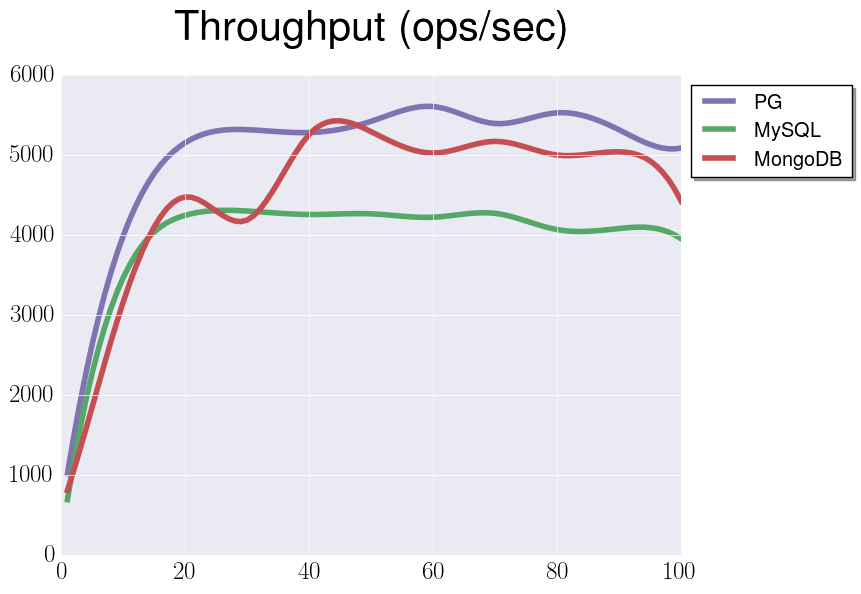
\includegraphics[width=0.75\textwidth,center]{benchmarks/update_btree_journaled_throughput.png}
    %\end{figure}
    %\end{center}
%\end{frame}

\begin{frame}
    \frametitle{}
    \begin{center}
    \vspace{10pt}
    \begin{figure}
        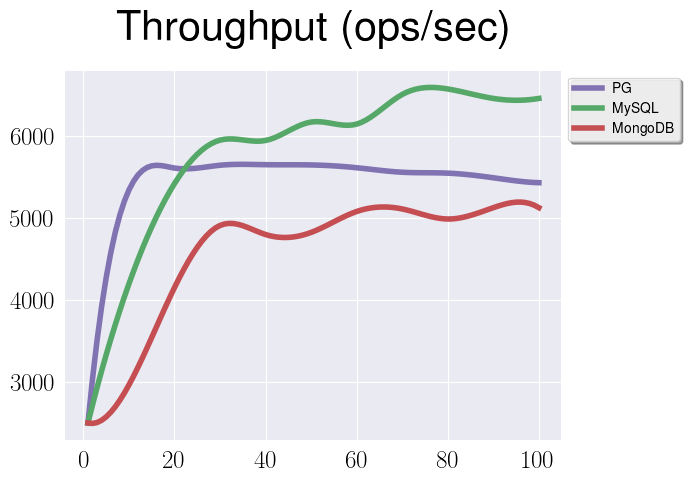
\includegraphics[width=0.8\textwidth,center]{benchmarks/update_btree_wal_size.png}
    \end{figure}
    \end{center}
\end{frame}

\begin{frame}
    \frametitle{}
    \begin{center}
        \textbf{Update 50\%, Select 50\%}
        \begin{itemize}[label={}]
            \item "large" document
            \item Update one field
        \end{itemize}
    \end{center}
\end{frame}

\begin{frame}
    \frametitle{}
    \begin{center}
    \vspace{10pt}
    \begin{figure}
        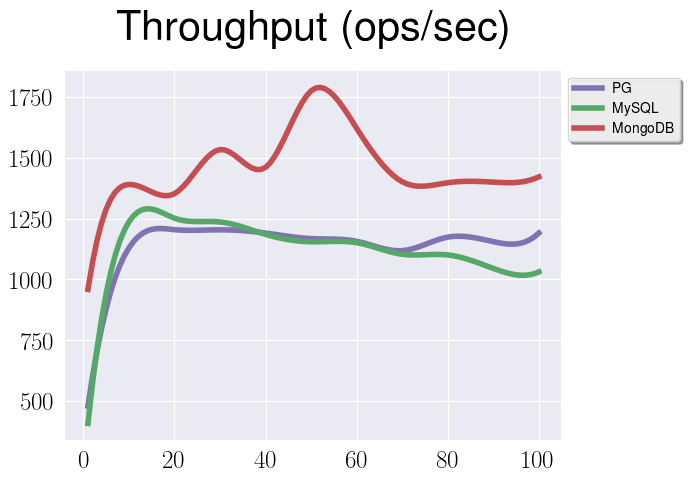
\includegraphics[width=0.8\textwidth,center]{benchmarks/update_btree_large_throughput.png}
    \end{figure}
    \end{center}
\end{frame}

%\begin{frame}
    %\frametitle{}
    %\begin{center}
    %%\vspace{-10pt}
    %\begin{figure}
        %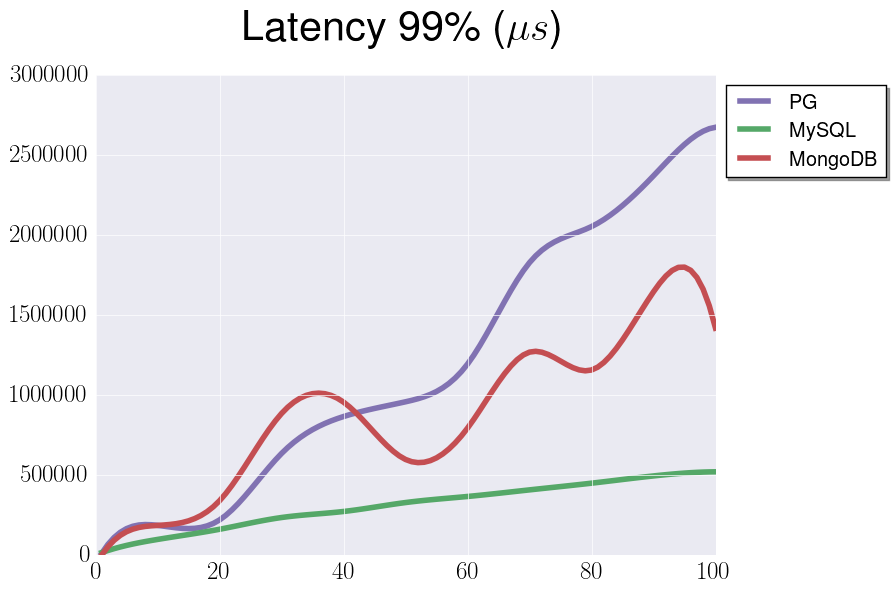
\includegraphics[width=0.75\textwidth,center]{benchmarks/update_btree_large_latency.png}
    %\end{figure}
    %\end{center}
%\end{frame}

\begin{frame}
    \frametitle{}
    \begin{center}
        \textbf{JSON vs JSONB}
        \begin{itemize}[label={}]
            \item "simple" document
            \item btree
            \item insert
        \end{itemize}
    \end{center}
\end{frame}

\begin{frame}
    \frametitle{}
    \begin{center}
    \vspace{10pt}
    \begin{figure}
        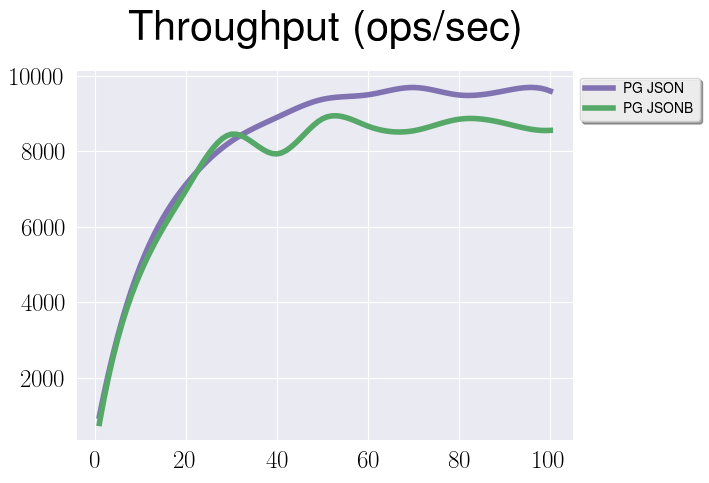
\includegraphics[width=0.8\textwidth,center]{benchmarks/postgresql_load_json_jsonb.png}
    \end{figure}
    \end{center}
\end{frame}

\begin{frame}
    \frametitle{}
    \begin{center}
        \textbf{JSON vs JSONB}
        \begin{itemize}[label={}]
            \item "simple" document
            \item btree
            \item select
        \end{itemize}
    \end{center}
\end{frame}

\begin{frame}
    \frametitle{}
    \begin{center}
    \vspace{10pt}
    \begin{figure}
        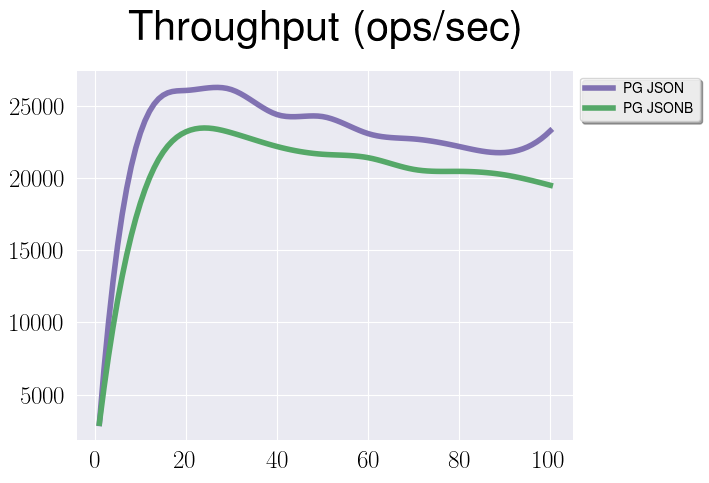
\includegraphics[width=0.8\textwidth,center]{benchmarks/postgresql_select_json_jsonb.png}
    \end{figure}
    \end{center}
\end{frame}

\begin{frame}
    \frametitle{}
    \begin{center}
        \textbf{SQL vs JSONB}
        \begin{itemize}[label={}]
            \item "simple" document
            \item btree
            \item insert
        \end{itemize}
    \end{center}
\end{frame}

\begin{frame}
    \frametitle{}
    \begin{center}
    \vspace{10pt}
    \begin{figure}
        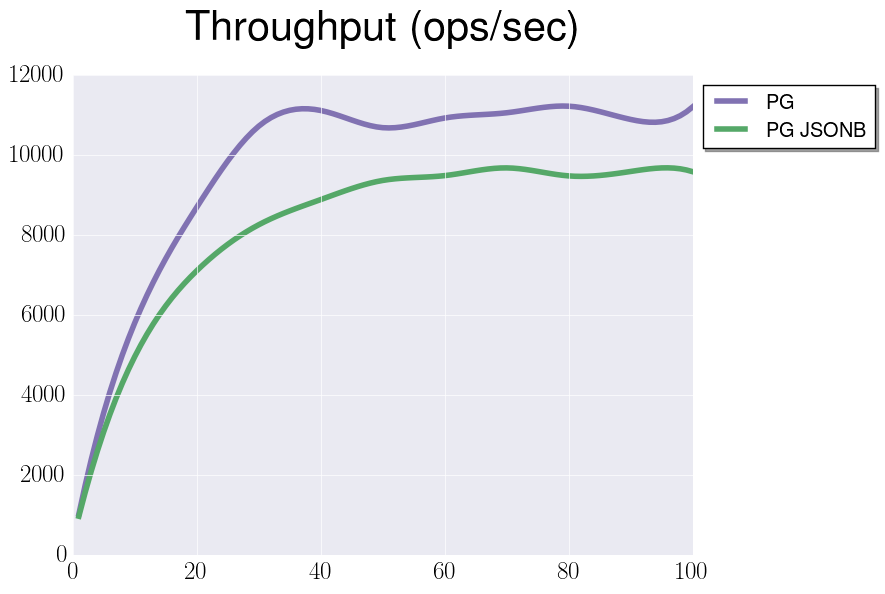
\includegraphics[width=0.8\textwidth,center]{benchmarks/postgresql_load_jsonb_jdbc.png}
    \end{figure}
    \end{center}
\end{frame}

\begin{frame}
    \frametitle{}
    \begin{center}
        \textbf{SQL vs JSONB}
        \begin{itemize}[label={}]
            \item "simple" document
            \item btree
            \item select
        \end{itemize}
    \end{center}
\end{frame}

\begin{frame}
    \frametitle{}
    \begin{center}
    \vspace{10pt}
    \begin{figure}
        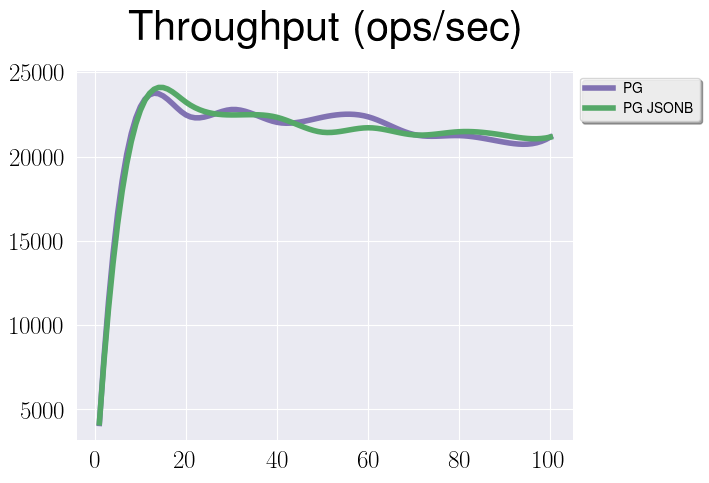
\includegraphics[width=0.8\textwidth,center]{benchmarks/postgresql_run_jsonb_jdbc.png}
    \end{figure}
    \end{center}
\end{frame}

\fontsize{13pt}{14}\selectfont
\section{How to bring it down accidentally?}
\fontsize{17pt}{18}\selectfont

\begin{frame}
    \frametitle{}
    \begin{center}
    %\vspace{-10pt}
    \begin{figure}
        
\includegraphics[width=0.55\textwidth,center]{wrong.jpg}
    \end{figure}
    \end{center}
\end{frame}

\begin{frame}
    \frametitle{}
    \begin{center}
        \begin{itemize}[label={\MVRightarrow}]
            \item Update one field of a document
            \item DETOAST of a document\\
                (select, constraints, procedures etc.)
            \item Reindex of an entire document
        \end{itemize}
    \end{center}
\end{frame}

\begin{frame}
    \frametitle{}
    \begin{center}
        \textbf{Document slice}
        \begin{itemize}[label={}]
            \item "large" document
            \item One field from a document
        \end{itemize}
    \end{center}
\end{frame}

\fontsize{17pt}{19}\selectfont
\begin{frame}
    \frametitle{}
    \begin{center}
    \inputminted[
        fontsize=\Large,
    ]{sql}{sql/detoast_overhead.sql}
    \end{center}
\end{frame}

\begin{frame}
    \frametitle{}
    \begin{center}
    \vspace{10pt}
    \begin{figure}
        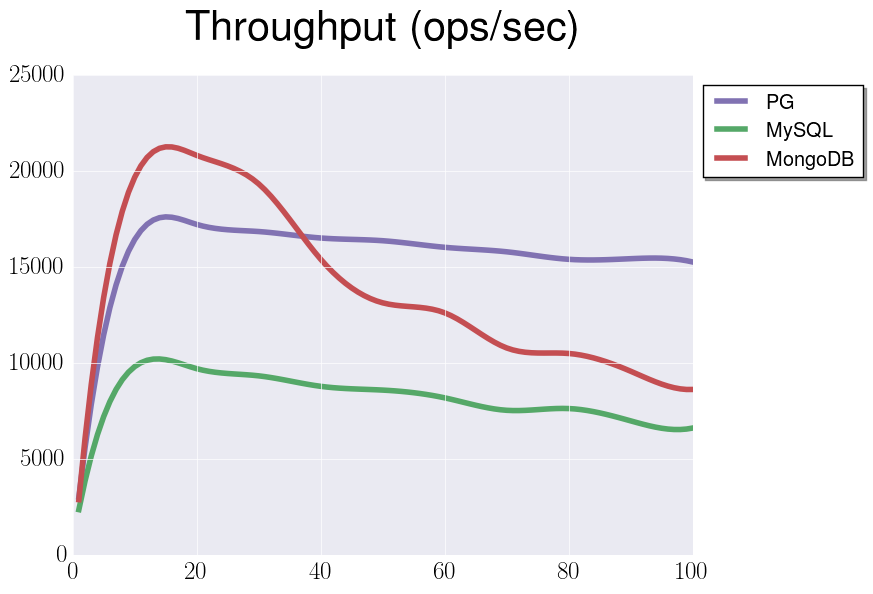
\includegraphics[width=0.8\textwidth,center]{benchmarks/select_slice_1_btree_throughput.png}
    \end{figure}
    \end{center}
\end{frame}

\begin{frame}
    \frametitle{}
    \begin{center}
        \textbf{Document slice}
        \begin{itemize}[label={}]
            \item "large" document
            \item 10 fields from a document
        \end{itemize}
    \end{center}
\end{frame}

\begin{frame}
    \frametitle{}
    \begin{center}
    \vspace{10pt}
    \begin{figure}
        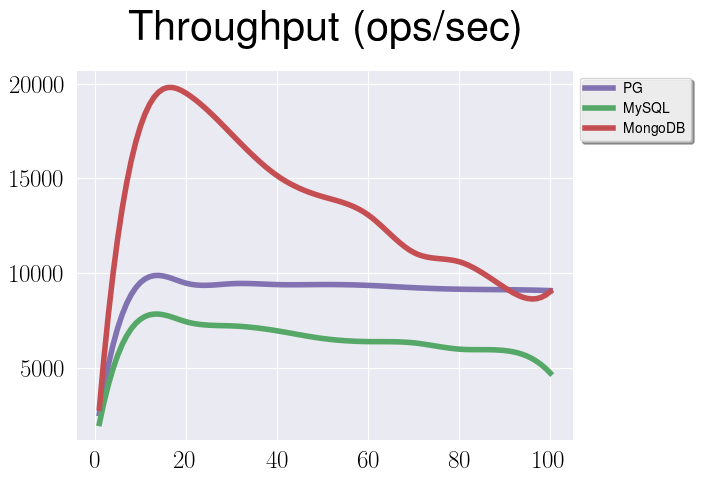
\includegraphics[width=0.8\textwidth,center]{benchmarks/select_slice_10_btree_throughput.png}
    \end{figure}
    \end{center}
\end{frame}

\fontsize{17pt}{19}\selectfont
\begin{frame}
    \frametitle{}
    \begin{center}
        \textbf{Document slice}
        \inputminted[
            fontsize=\Large,
        ]{sql}{sql/unwrap.sql}
    \end{center}
\end{frame}

\usebackgroundtemplate{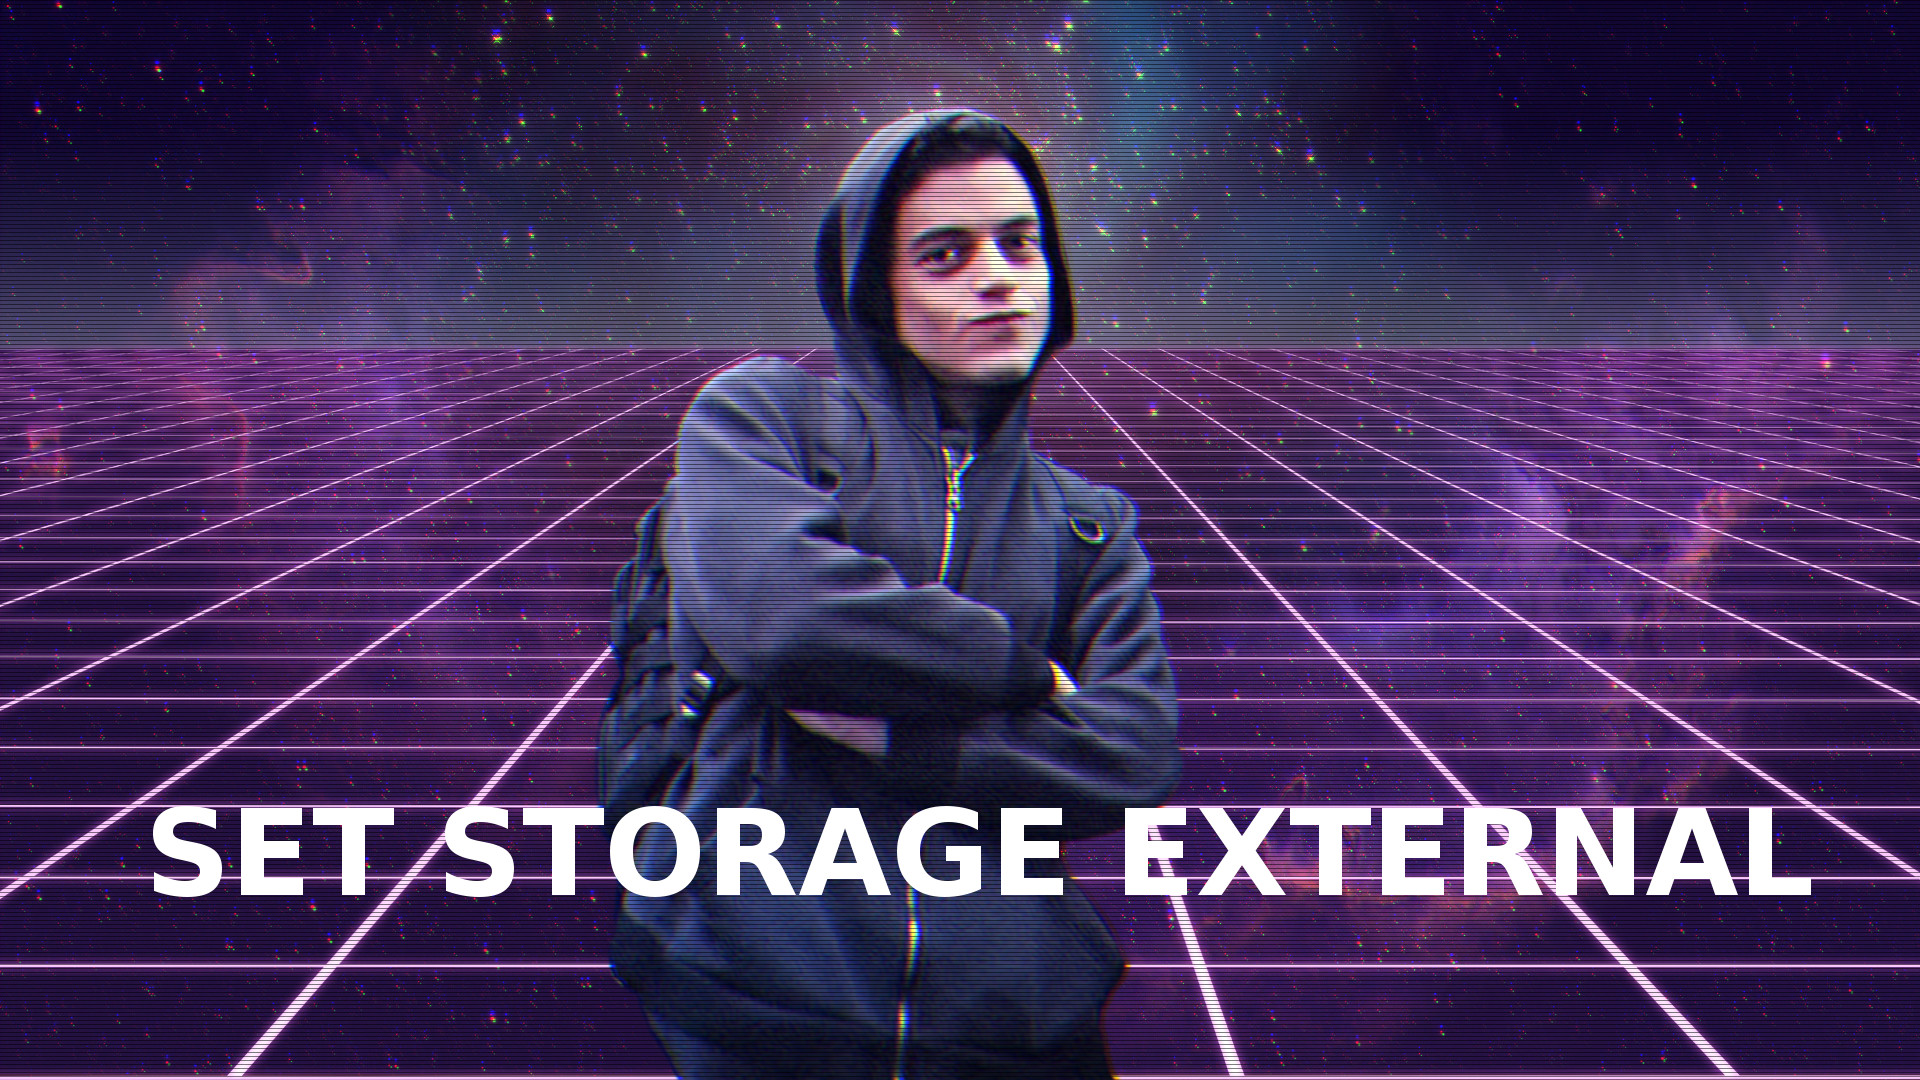
\includegraphics[width=\paperwidth]{hack.jpg}}%
\begin{frame}
    \frametitle{}
\end{frame}

%\usebackgroundtemplate{
\includegraphics[width=\paperwidth]{slide_background.png}}
\setbeamertemplate{background canvas}{
\begin{tikzpicture}
    \clip (0,0) rectangle (\paperwidth,\paperheight);
    \fill[color=orange] (4cm, \paperheight-6pt) rectangle (\paperwidth-4cm,\paperheight);
\end{tikzpicture}
}

\begin{frame}
    \frametitle{}
    \begin{center}
        \textbf{TOAST\_TUPLE\_THRESHOLD}
        \begin{itemize}[label={}]
            \item "simple" document
            \item 40 threads
            \item different document size
            \item select
        \end{itemize}
    \end{center}
\end{frame}

\begin{frame}
    \frametitle{}
    \begin{center}
    \vspace{10pt}
    \begin{figure}
        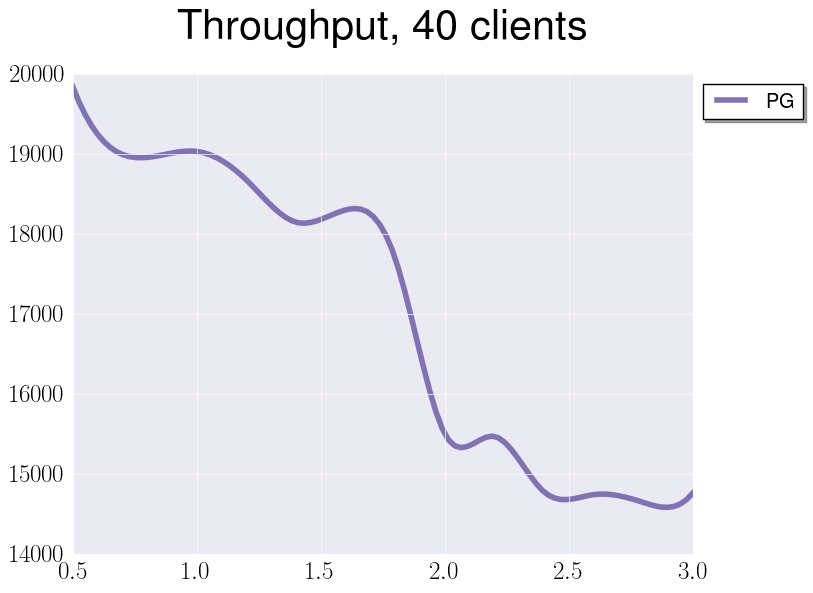
\includegraphics[width=0.75\textwidth,center]{benchmarks/workload_c_toast.png}
    \end{figure}

    \end{center}
\end{frame}

\begin{frame}
    \frametitle{}
    \begin{center}
        \textbf{Select, GIN}
        \begin{itemize}[label={}]
            \item "simple" document
            \item jsonb\_path\_ops
            \item where data @> jsonb\_build\_object('key', 'value')
        \end{itemize}
    \end{center}
\end{frame}

\begin{frame}
    \frametitle{}
    \begin{center}
    \vspace{10pt}
    \begin{figure}
        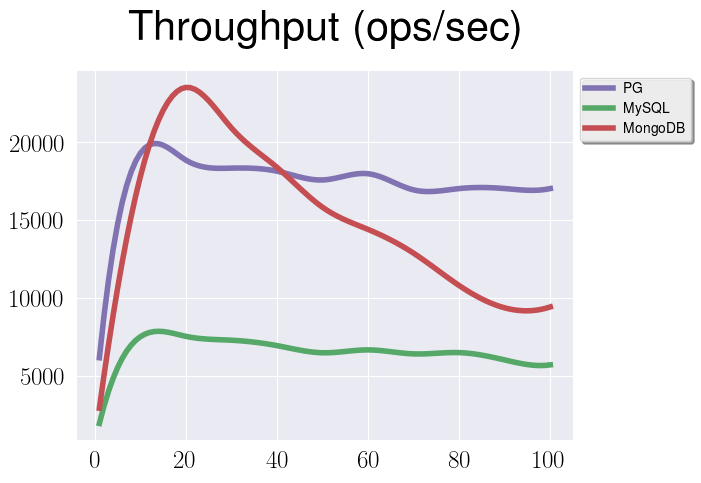
\includegraphics[width=0.8\textwidth,center]{benchmarks/select_jsonb_path_ops_no_parse_throughput.png}
    \end{figure}
    \end{center}
\end{frame}
\note{
    for parse - `jsonb\_from\_cstring`
    for no parse - `just datum\_to\_jsonb`
}

%\begin{frame}
    %\frametitle{}
    %\begin{center}
        %\textbf{Jsonb array}
    %\end{center}
%\end{frame}

%\begin{frame}
    %\frametitle{}
    %\begin{center}
        %\textbf{Jsonb type convertion}
    %\end{center}
%\end{frame}

%\begin{frame}
    %\frametitle{}
    %\begin{center}
        %\textbf{Index maintaining}
    %\end{center}
%\end{frame}

%\begin{frame}
    %\frametitle{}
    %\begin{center}
        %\textbf{Cluster}
    %\end{center}
%\end{frame}

%\begin{frame}
    %\frametitle{}
    %\begin{center}
    %\vspace{-10pt}
    %\textbf{Вставка записей}
    %\end{center}
%\end{frame}

%\begin{frame}
    %\frametitle{}
    %\begin{center}
    %\vspace{-10pt}
    %\textbf{Вставка и обновление}
    %\end{center}
%\end{frame}

%\begin{frame}
    %\frametitle{}
    %\begin{center}
    %\vspace{-10pt}
    %\textbf{Чтение последних}
    %\end{center}
%\end{frame}

%\begin{frame}
    %\frametitle{}
    %\begin{center}
    %\vspace{-10pt}
    %\textbf{Чтение, изменение, запись}
    %\end{center}
%\end{frame}

\begin{frame}[fragile]
    \frametitle{}
    \vspace{10pt}
    \begin{itemize}[leftmargin=*, label={\MVRightarrow}]
        \item <+-> Jsonb is more that good for many use cases
        \item <+-> Benchmarks above are only "hints"
        \item <+-> You need your own tests
    \end{itemize}
\end{frame}
\note{
    чтение, поиск и вставка - "правильный вид нагрузки" для реляционной базы данных по мнению финна Markus Winand
}

%\usebackgroundtemplate{
\includegraphics[width=\paperwidth]{title_background.png}}

\fontsize{17pt}{18}\selectfont
\begin{frame}
  \vspace*{2.5cm}
  %\column{0.3\textwidth}
  %\column{0.7\textwidth}
  \begin{minipage}[b][\paperheight]{\textwidth}
  \begin{center}

      %\raggedright%
      \linespread{1.0}%
      \usebeamerfont{title}%
      \usebeamercolor[fg]{title}%
      \if@noSmallCapitals%
        Questions?
      \else%
        \scshape{\color{black} Questions?}%
      \fi%
      \vspace*{0.3em}

      \usebeamerfont{subtitle}%
      \fontsize{13pt}{14}\selectfont
      \usebeamercolor[fg]{subtitle}%
        \begin{itemize}[label={}]
            \item {\color{black} \github\ github.com/erthalion}
            \item {\color{black} \twitter\ @erthalion}
            \item {\color{black}\email\ 9erthalion6 at gmail dot com}
        \end{itemize}
      \vspace*{2.5em}%

    \vfill
    \vspace*{2em}
  \end{center}
  \end{minipage}

\end{frame}

\fontsize{17pt}{19}\selectfont
\begin{frame}
    \frametitle{}
    \begin{center}
    \inputminted[
        fontsize=\Large,
    ]{json}{sql/update_document_data.json}
    \end{center}
\end{frame}

\fontsize{17pt}{19}\selectfont
\begin{frame}
    \frametitle{}
    \begin{center}
    \inputminted[
        fontsize=\Large,
    ]{sql}{sql/update_document.sql}
    %\inputminted[
        %fontsize=\large,
    %]{bash}{sql/update_document.sh}
    \end{center}
\end{frame}

\begin{frame}
    \frametitle{}
    \begin{center}
        \textbf{Scalability}
        \begin{itemize}[label={}]
            \item "simple" document
            \item m4.large
            \item m4.xlarge
            \item m4.2xlarge
        \end{itemize}
    \end{center}
\end{frame}

\begin{frame}
    \frametitle{}
    \begin{center}
    %\vspace{-10pt}
    \begin{figure}
        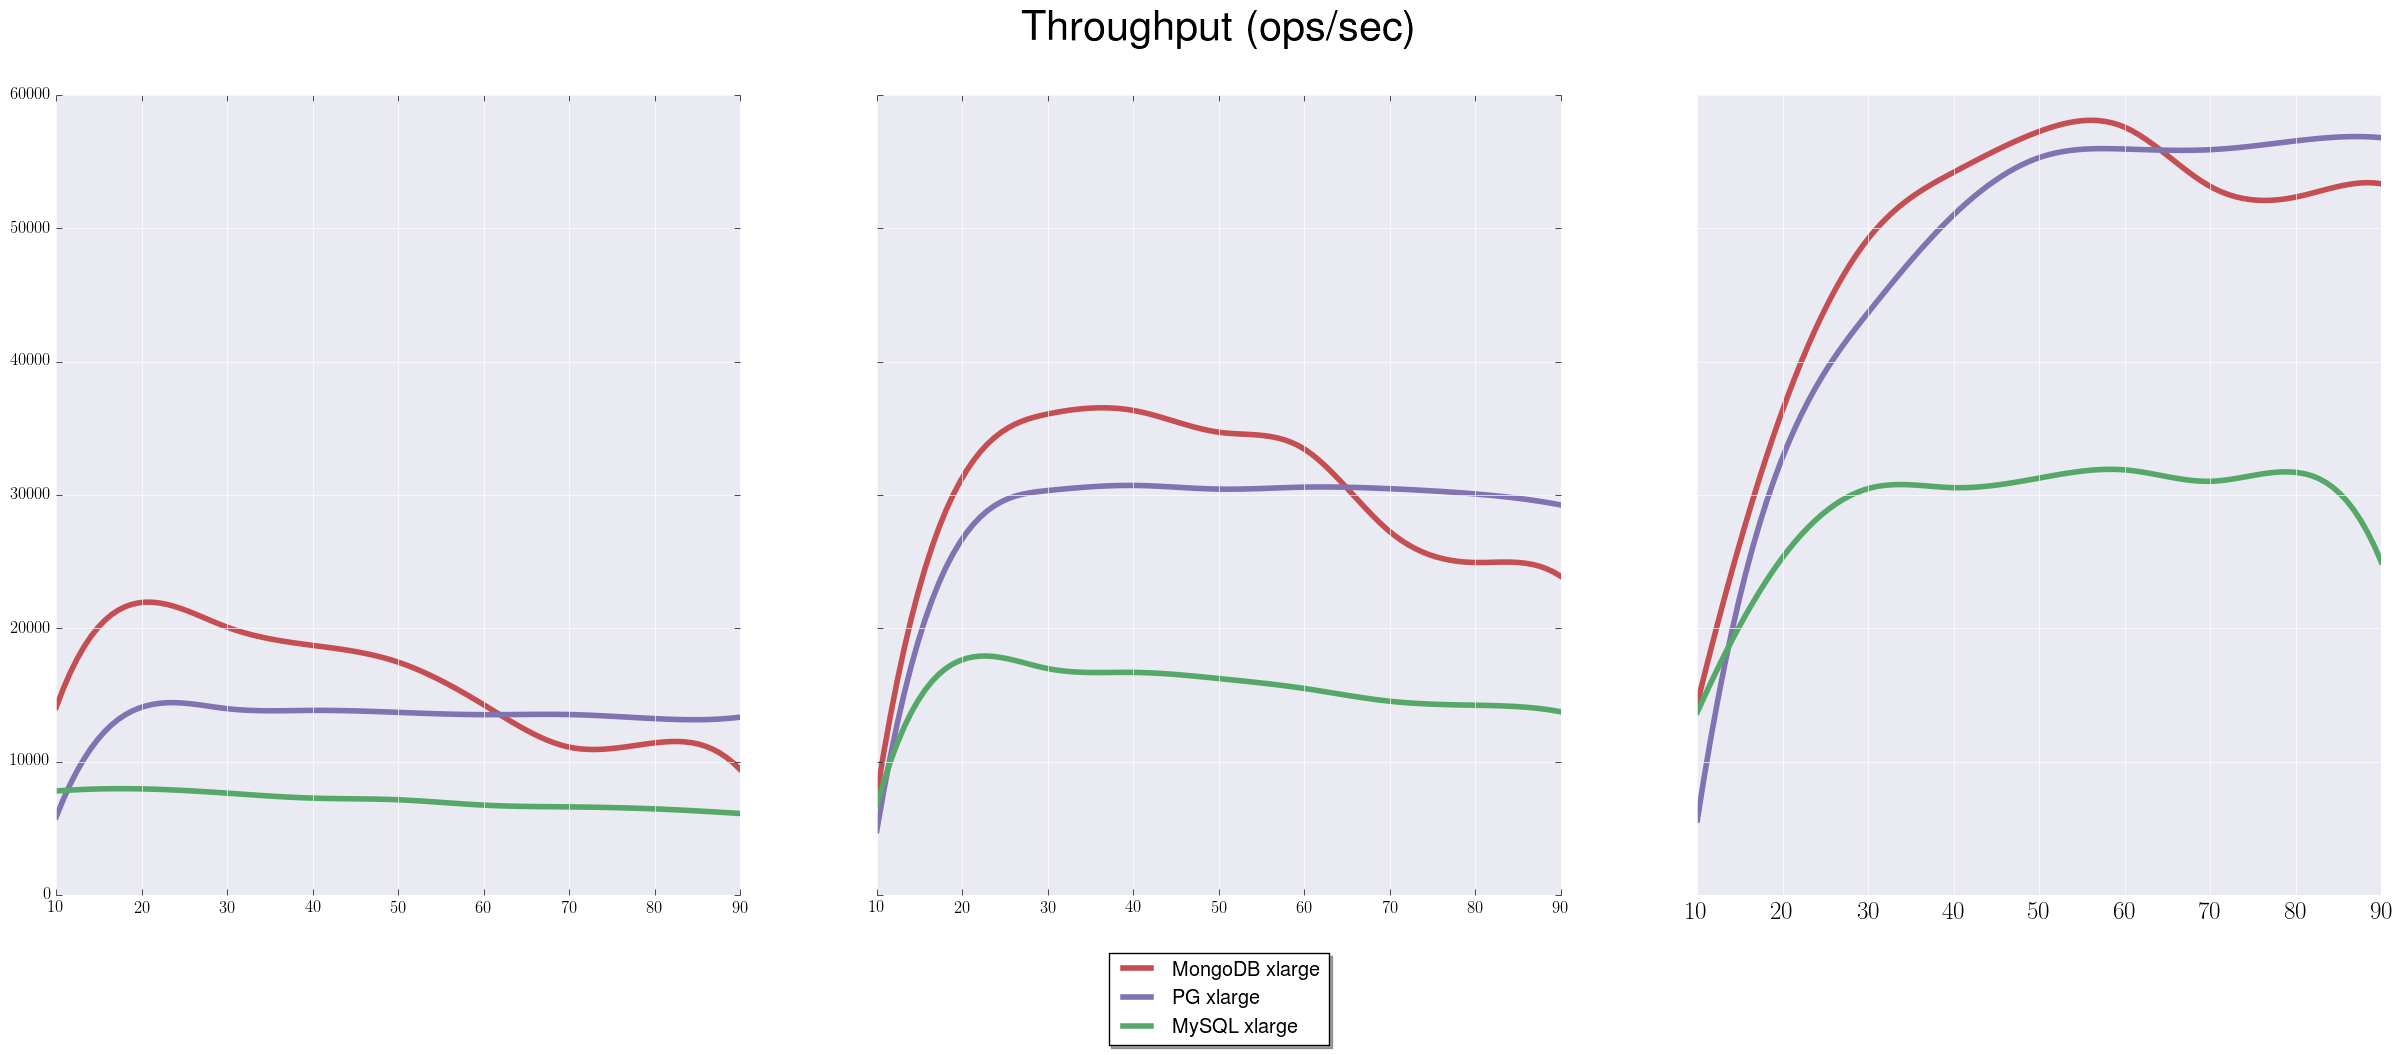
\includegraphics[height=8cm,width=1.1\textwidth,center]{benchmarks/scalability_select_throughput.png}
    \end{figure}
    \end{center}
\end{frame}

\end{document}
